\chapter{Trigger Analysis $\&$ Characterization}
\label{chap:trigStudy}

The following chapter discusses the experimental testing and characterization of the trigger once installed in the detector. To maximize the sensitivity of the detector, it is crucial that the behaviour of the trigger be well understood. Using a system of light injection, the statistical efficiency of the \gls{dtm} is analysed. The \gls{dtm}'s efficiency at the trigger threshold crossing will be used to set the event sorting thresholds for energy regions as discussed in Section \ref{sec:triggerAlgorithm}.
\section{AARF Light Injection}
\label{sec:aarfs}
The acrylic reflector and fibre optics (\gls{aarf}) system serves as a permanent light injection system for the \gls{deap3} detector. The \gls{aarf}s are designed to calibrate the charge generated by a single photon at the beginning of a data run. Additionally the \gls{aarf}s are used for calibration of \gls{pmt} timing and detector stability with time \cite{alaisterThesis}.

The \gls{aarf} system uses aluminium coated acrylic reflectors to inject 435 nm \gls{led} light, over an acrylic fibre onto a host \gls{pmt}, as shown in Fig. \ref{Fig:AARFImage}. \gls{deap3} is outfitted with 20 \gls{pmt} \gls{aarf}s with an additional two reflectors in the neck of the detector with no host \gls{pmt}. In a \gls{pmt} \gls{aarf} 97$\%$ of the injected light in found in the host \gls{pmt}, with only $3\%$ reflected onto its surrounding neighbours \cite{alaisterThesis}. The neck \gls{aarf}s, without a host \gls{pmt}, allows for more evenly distribution of light over the detector.


 \begin{figure}
 \centering
 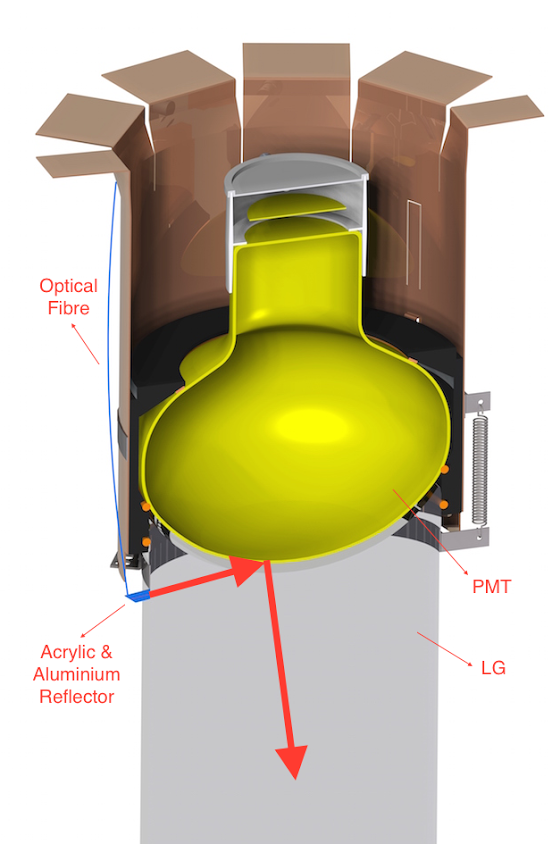
\includegraphics[height = 0.5\paperheight]{PMTAARFCartoon}
 \caption{Rendering of the light injection system for a \gls{pmt} \gls{aarf}. Light from a 435 nm \gls{led} is passed over an acrylic optical fibre and reflected off an aluminium coated acrylic reflector onto the host \gls{pmt}.}
 \label{Fig:AARFImage}
 \end{figure}
 
\section{Efficiency Study}
Light injection using the \gls{aarf} system was used for finding the efficiency of the \gls{dtm}. The triggering algorithm is as follows:

\begin{enumerate}
\item A \gls{dtm} periodic trigger is sent to the \gls{aarf}s
\item The \gls{aarf}s send an external pulse to the \gls{dtm} causing the \gls{v1720} digitizers to begin recording
\item The \gls{aarf} \gls{led} pulses, injecting light into the detector
\item The \gls{dtm} integrates the charge from the \gls{pmt}s, if the set threshold for total short energy is meet, a \gls{dtm} event will be recorded.
\item Every \gls{aarf} event's integrated \gls{v1720} charge is recorded in a histogram, if a \gls{dtm} event occurs a second histogram is filled with the event indicating the events that passed the threshold.
\end{enumerate}
%Two types of periodic triggers were used; an exponential periodic trigger (Exponential 1) which fires following an exponential distribution; and a periodic trigger (Periodic 0) which fires at a set frequency. 
Using this trigger scheme, the outputs and settings of which are given in Table \ref{Table:trigSchemePeriodic}, the efficiency at a threshold crossing can be analysed.


%\begin{table}[h]
%\centering
%\caption{Triggers and output setting used for periodic light injection efficiency study corresponding to run types 301-302 (see Table \ref{Table:runDescrip}).}
%\vspace{0.2cm}
%\begin{tabular}{c	c	c	c	c}
%\hline
%\hline
%\textbf{Trigger}&		\textbf{Rate (Hz)}&		\textbf{Outputs}&		\textbf{Prescaler}\\
%\hline
%Periodic 1&		56&		V1720&						1\\
%Exponential 0&	1500&		V1720, Calib, AARF&			1 \\
%Exponential 0&	1500&		V1720,V1740, Calib, AARF&	5 \\
%ADC High Energy&	N/A&		&						1 \\
%ADC High Energy&	N/A&		DTM&					100\\
%\hline
%\hline
%\end{tabular}
%\label{Table:trigSchemeExp}
%\end{table}

\begin{table}[h]
\centering
\caption{Triggers and output setting used for periodic light injection efficiency study corresponding to run types 304-306 (see Table \ref{Table:runDescrip}).}
\vspace{0.2cm}
\begin{tabular}{c	c	c	c	c}
\hline
\hline
\textbf{Trigger}&		\textbf{Rate (Hz)}&		\textbf{Outputs}&		\textbf{Prescaler}\\
\hline
Periodic 0&			1500&		V1720, Calib, AARF&					1 \\
Periodic 0&			1500&		V1720,V1740, Calib, AARF&			5 \\
Periodic 1&			56&		V1720&								1 \\
ADC High Energy&	N/A&		&									1 \\
ADC High Energy&	N/A&		DTM&								100\\
\hline
\hline
\end{tabular}
\label{Table:trigSchemePeriodic}
\end{table}

In this study \gls{fprompt} is not taken into account and therefore a trigger will be generated by the \gls{dtm} for any event that has the set threshold charge integrated over a set number of clocks (denoted as short window in Table \ref{Table:runDescrip}).


\subsection{Data Taking}

Data runs were taken at three different \gls{dtm} thresholds where it is estimate the low, medium, and high energy cuts will be made for the trigger level \gls{psd}. The runs were then preformed for several different intensities of the \gls{aarf}s, ensuring good statistics across the threshold crossing region. The \gls{aarf} light is very prompt, as is to be expected; Fig. \ref{Fig:wf_Fprompt_low} - \ref{Fig:wf_Fprompt_high} show typical \gls{ass} \gls{dtm} waveforms for three \gls{aarf} intensities and the associated charge-\gls{fprompt} relation. The charge is given in photo electrons (\gls{pe}) measured by the \gls{v1720}s utilizing photon counting to reduce uncertainty. The data run summaries are given in Table \ref{Table:runDescrip}.

\begin{table}[h]
\centering
\caption{Data run descriptions for trigger efficiency study. Run numbers sharing a run type denote a change in \gls{aarf} intensity only.}
\vspace{.2cm}

\begin{tabular}{c	c	c	c	c}
\hline
\hline

\textbf{Run}&	\textbf{Type}&		\textbf{AARF}& \textbf{DTM Threshold}&	\textbf{Short}\\
&	&		\textbf{Intensity}& \textbf{(ADC)}&	\textbf{Window (ns)}\\

\hline
15826&	304&	1270&		1400 &	128\\
15827&	304&	1300&		1400 &	128\\
15828&	305&	1530&		6000 &	128\\
15829&	305&	1560&		6000 &	128\\
15830&	306&	1835&		15000 &	128\\
15831&	306&	1870&		15000 &	128\\

\hline
\hline
\end{tabular}
\label{Table:runDescrip}
\end{table}

The data runs for a single \gls{dtm} threshold are combined into a single histogram to ensure a range of charge near the \gls{dtm} threshold. These histograms are plotted in superimposed pairs in Fig. \ref{Fig:effHists1400} - \ref{Fig:effHists15000}.

\clearpage
\begin{figure}
    \centering
    \begin{subfigure}[t]{0.48\textwidth}
		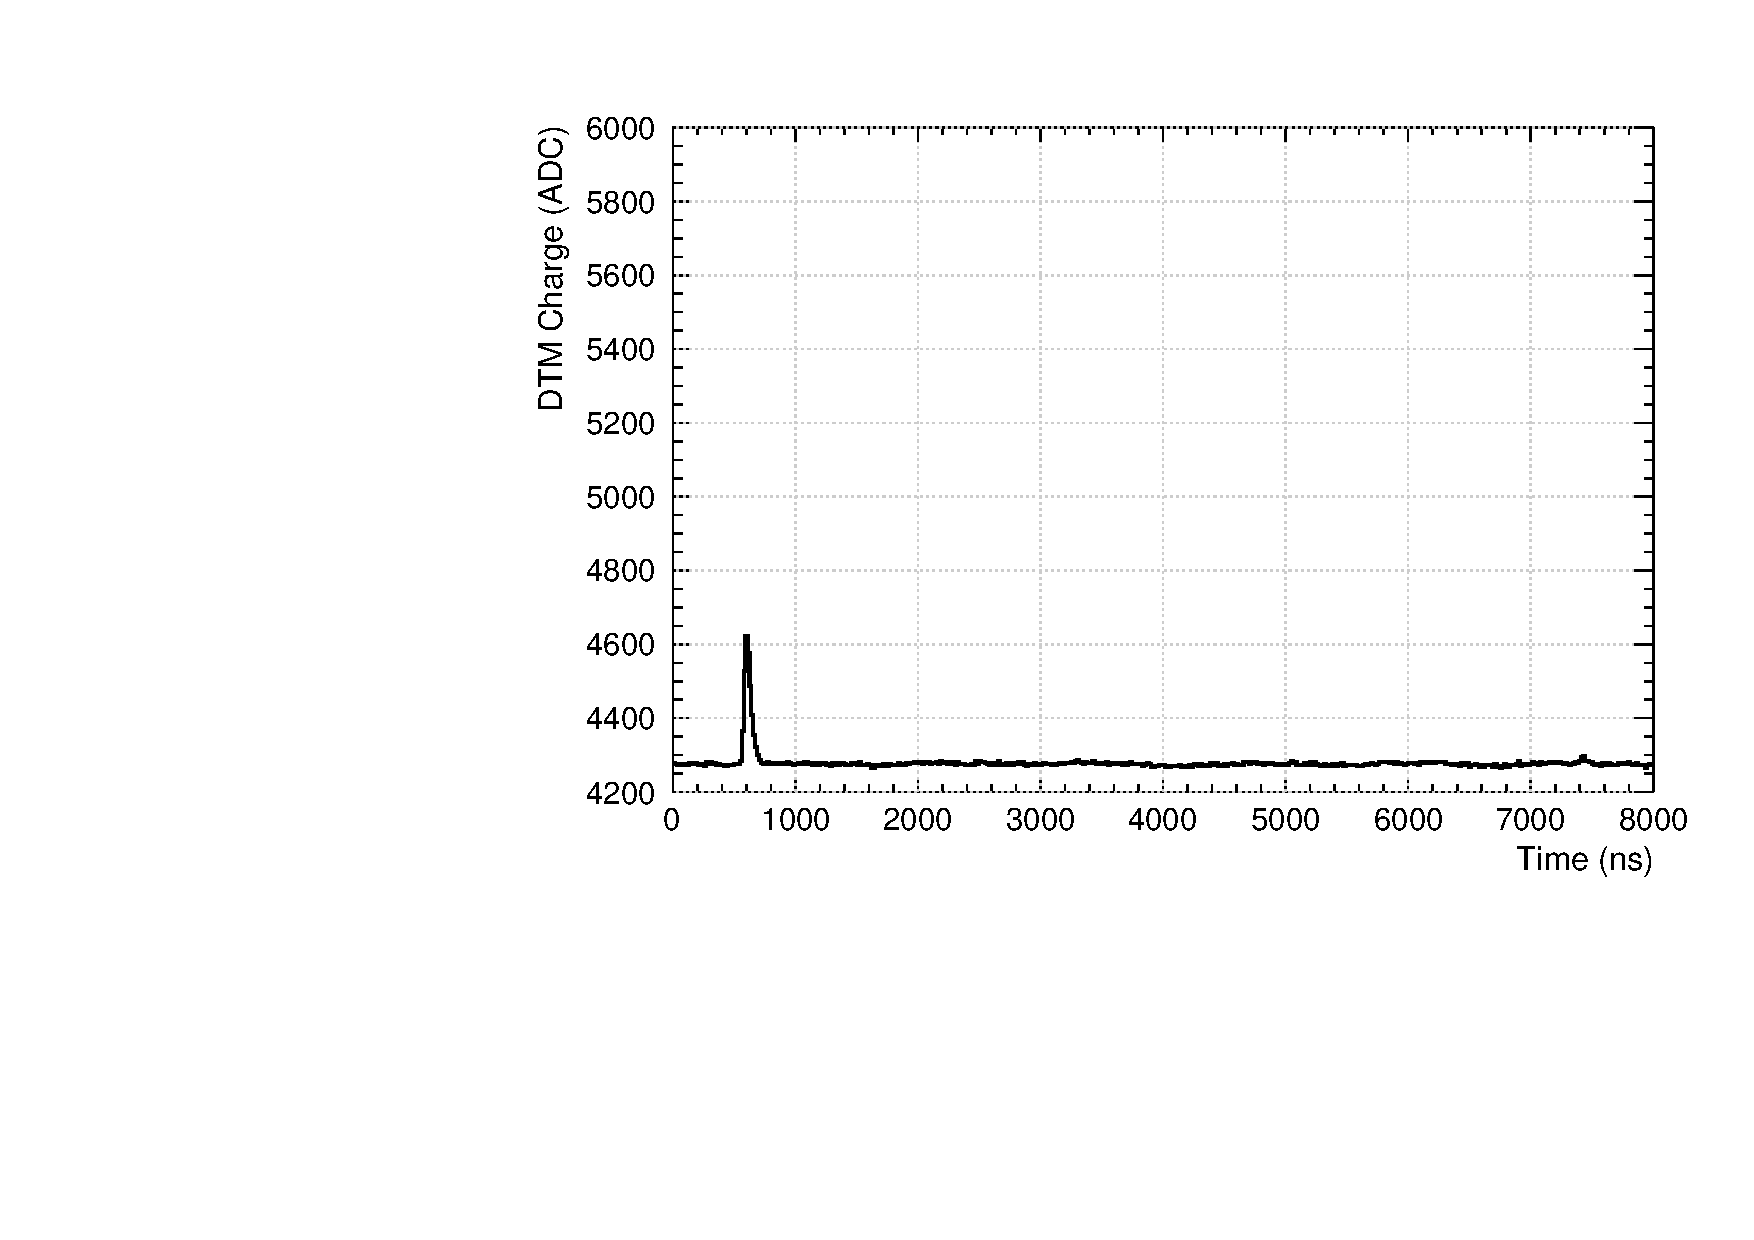
\includegraphics[width=\textwidth]{results/dtmWF_15826_1306}
		%\caption{Typical \gls{aarf} \gls{dtm} waveform for an intensity of 1270.}
		\label{Fig:wfShort} 
    \end{subfigure}
    ~ %add desired spacing between images, e. g. ~, \quad, \qquad, \hfill etc. 
      %(or a blank line to force the subfigure onto a new line)
    \begin{subfigure}[t]{0.48\textwidth}
        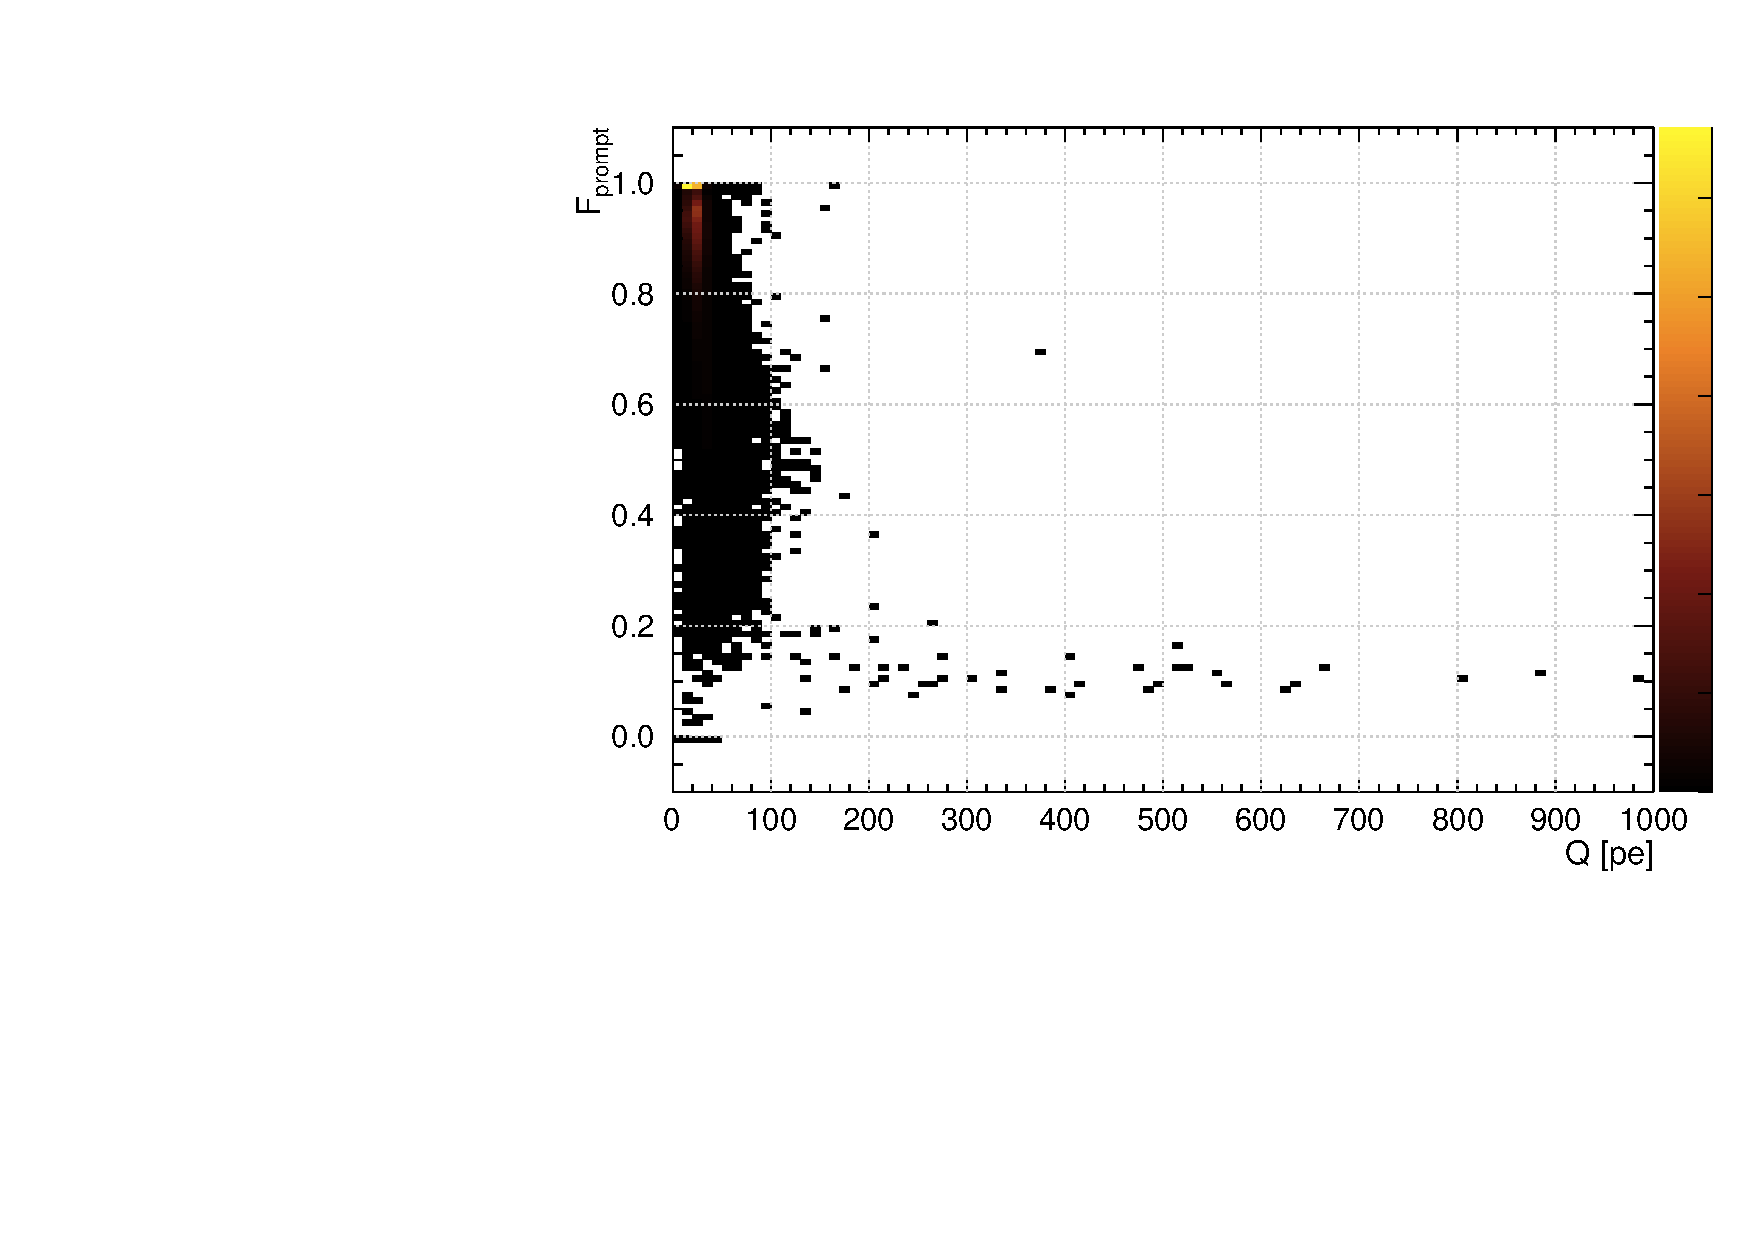
\includegraphics[width=\textwidth]{results/fprompt_015826}
        %\caption{Fprompt}
        \label{Fig:fprompt15826}
    \end{subfigure}
    \caption{\textbf{Left:} Typical \gls{aarf} \gls{dtm} waveform for an intensity of 1270. \textbf{Right:} \gls{fprompt} against number of photo electrons recorded per event at an \gls{aarf} intensity of 1270}
	\label{Fig:wf_Fprompt_low}
\end{figure}


\begin{figure}
    \centering
    \begin{subfigure}[t]{0.48\textwidth}
		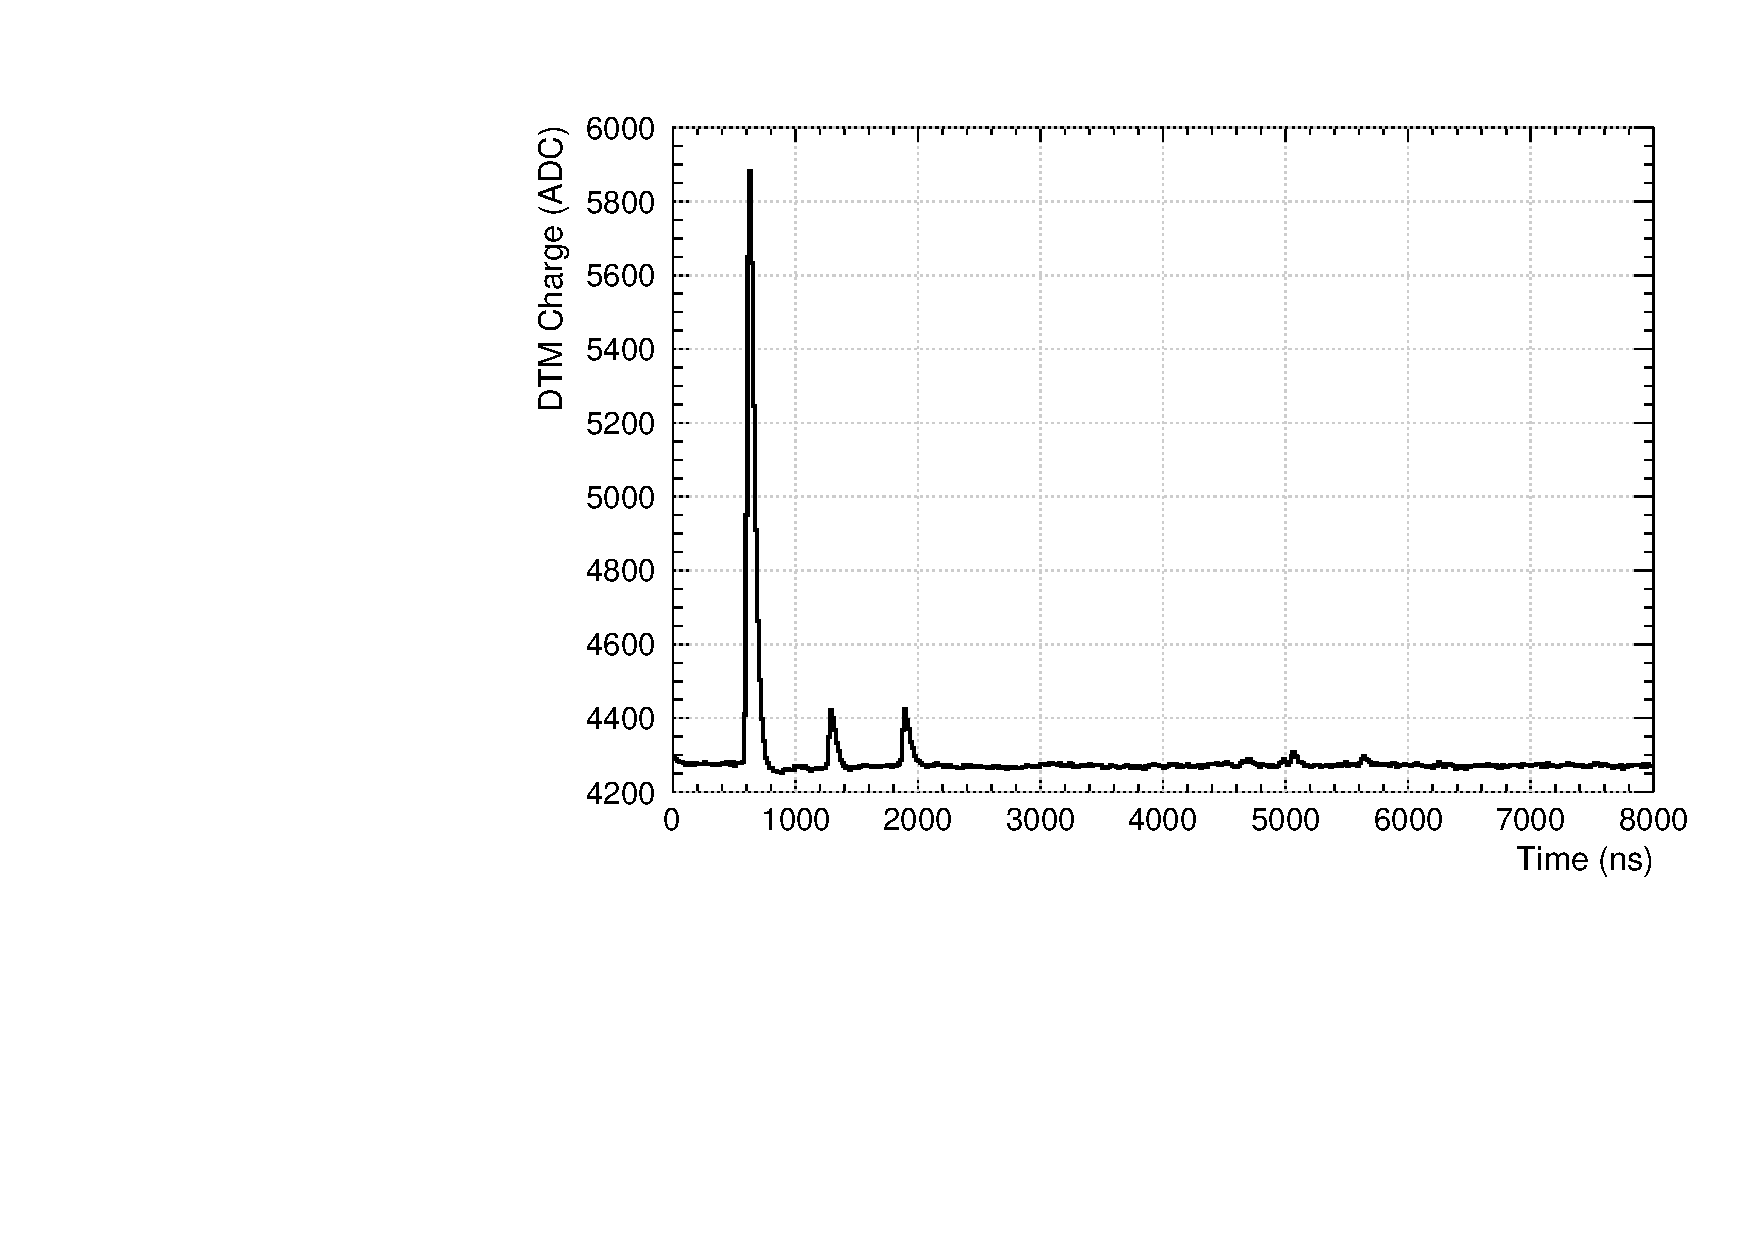
\includegraphics[width=\textwidth]{results/dtmWF_15828_405}
		%\caption{Typical \gls{aarf} \gls{dtm} waveform for an intensity of 1530.}
		\label{Fig:wfMedium}
    \end{subfigure}
    ~ %add desired spacing between images, e. g. ~, \quad, \qquad, \hfill etc. 
      %(or a blank line to force the subfigure onto a new line)
    \begin{subfigure}[t]{0.48\textwidth}
        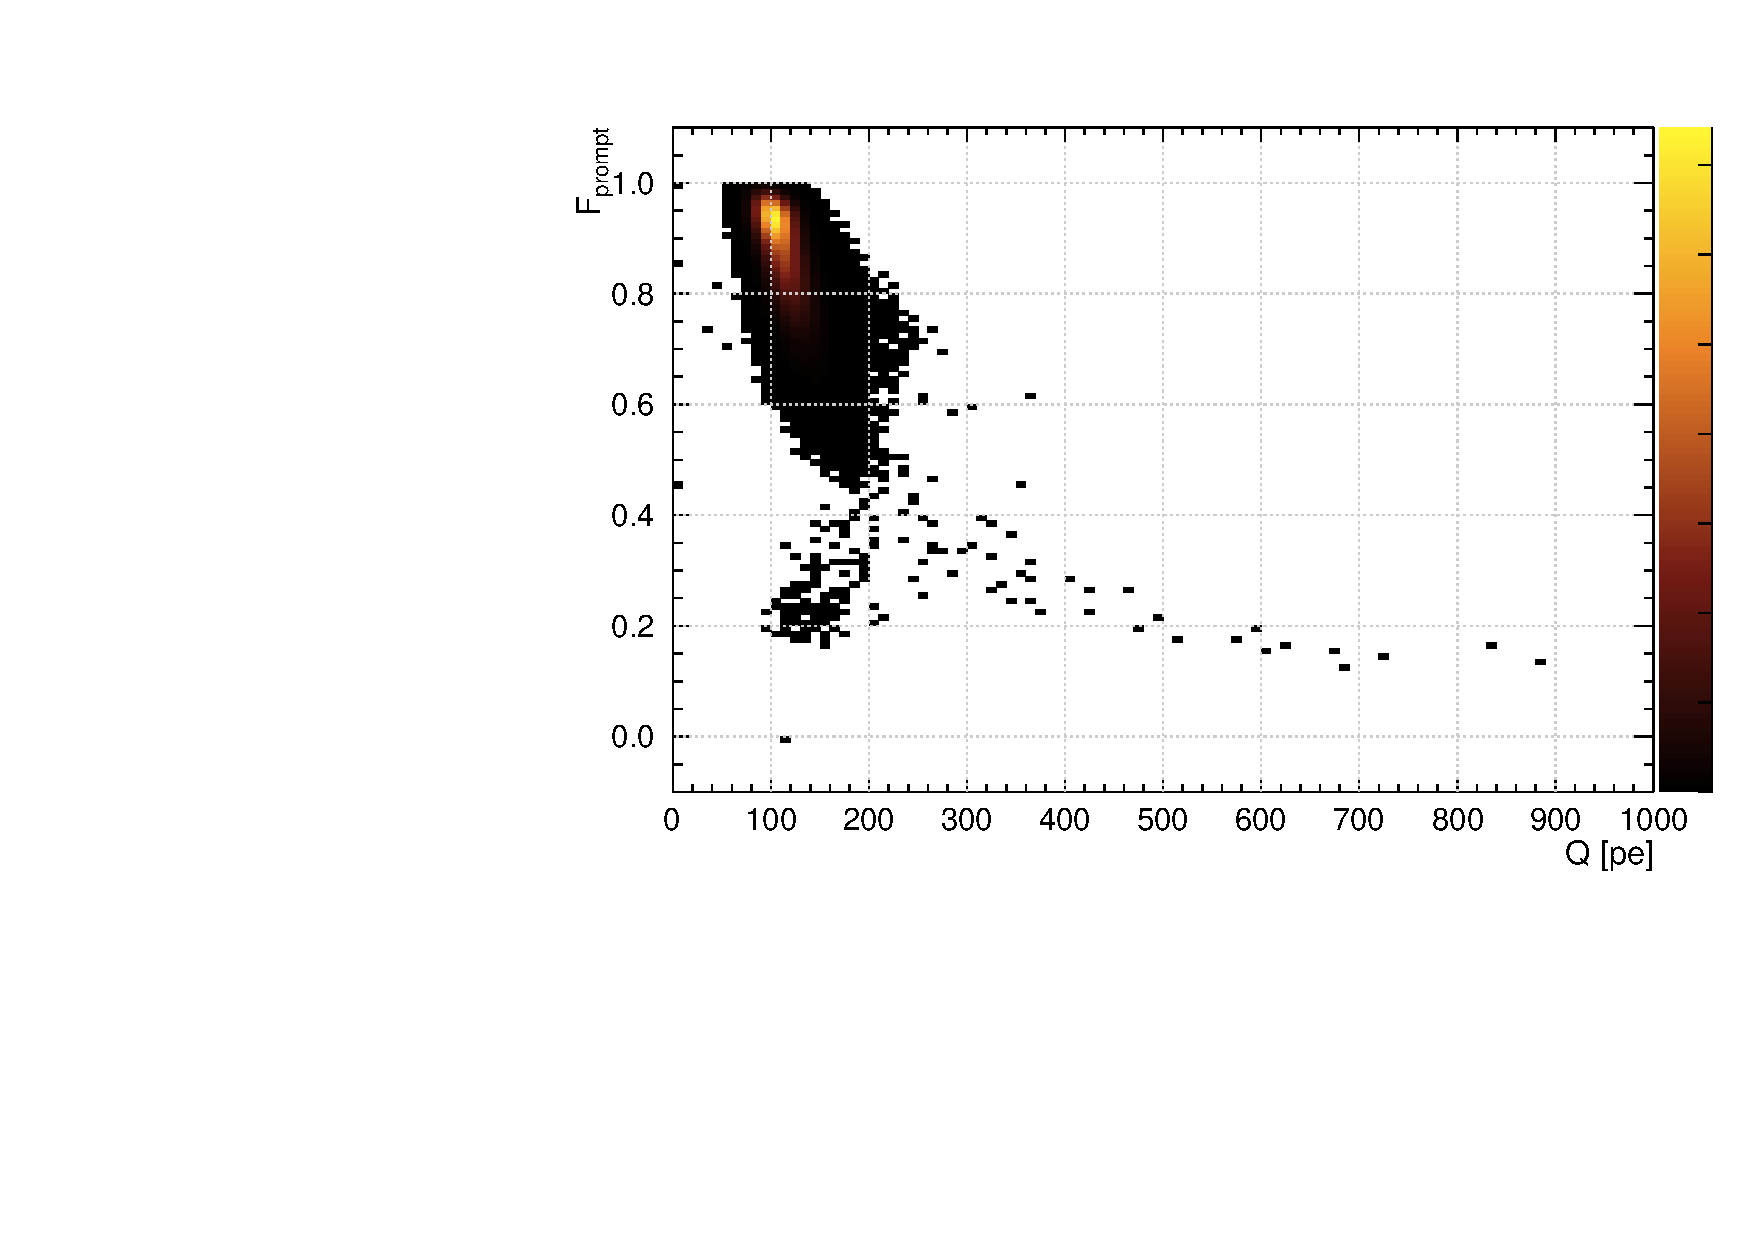
\includegraphics[width=\textwidth]{results/fprompt_015828}
        %\caption{A tiger}
        \label{Fig:fprompt15828}
    \end{subfigure}
    \caption{\textbf{Left:} Typical \gls{aarf} \gls{dtm} waveform for an intensity of 1530. \textbf{Right:} \gls{fprompt} against number of photo electrons recorded per event at an \gls{aarf} intensity of 1530}
    \label{Fig:wf_Fprompt_mid}
\end{figure}

\begin{figure}
    \centering
    \begin{subfigure}[t]{0.48\textwidth}
		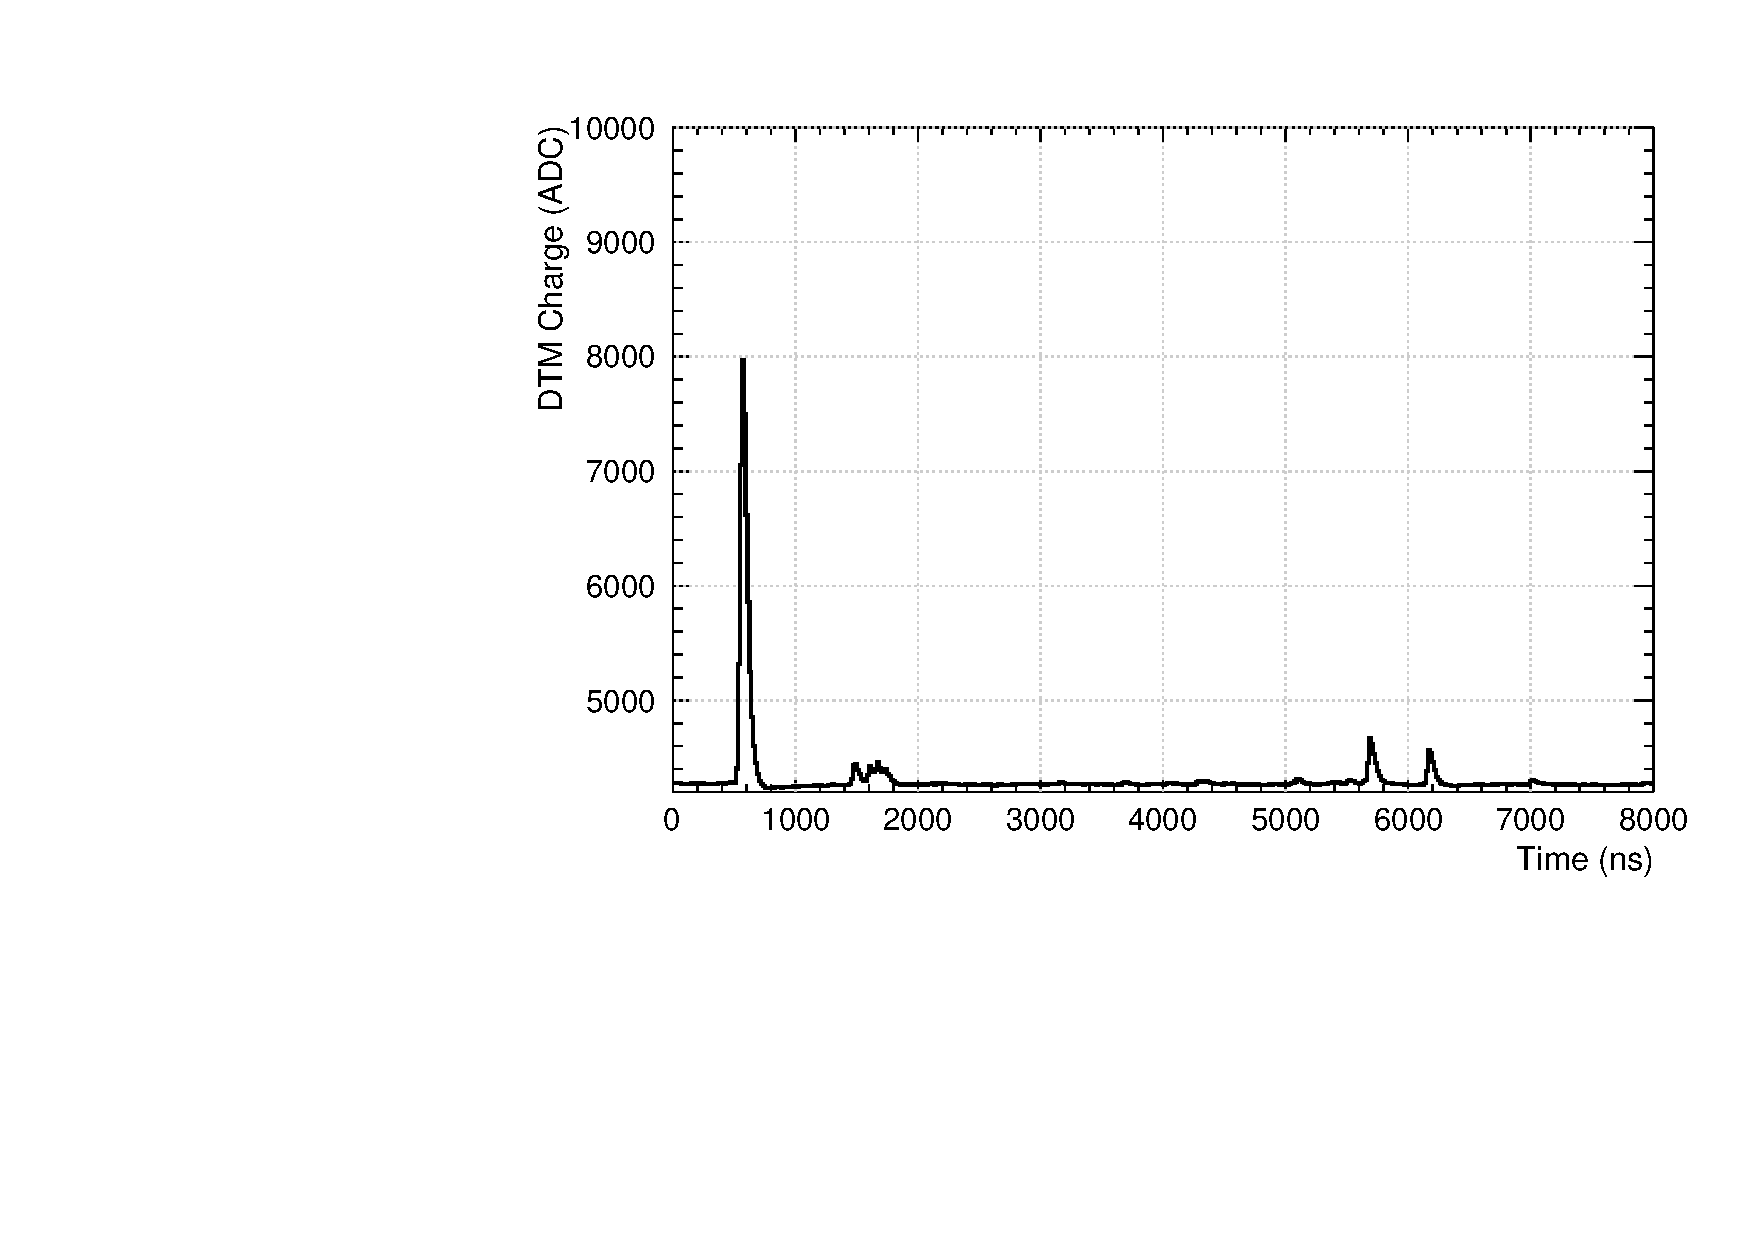
\includegraphics[width=\textwidth]{results/dtmWF_15831_718}
		%\caption{Typical \gls{aarf} \gls{dtm} waveform for an intensity of 1870.}
		\label{Fig:wfHigh}
    \end{subfigure}
    ~ %add desired spacing between images, e. g. ~, \quad, \qquad, \hfill etc. 
      %(or a blank line to force the subfigure onto a new line)
    \begin{subfigure}[t]{0.48\textwidth}
        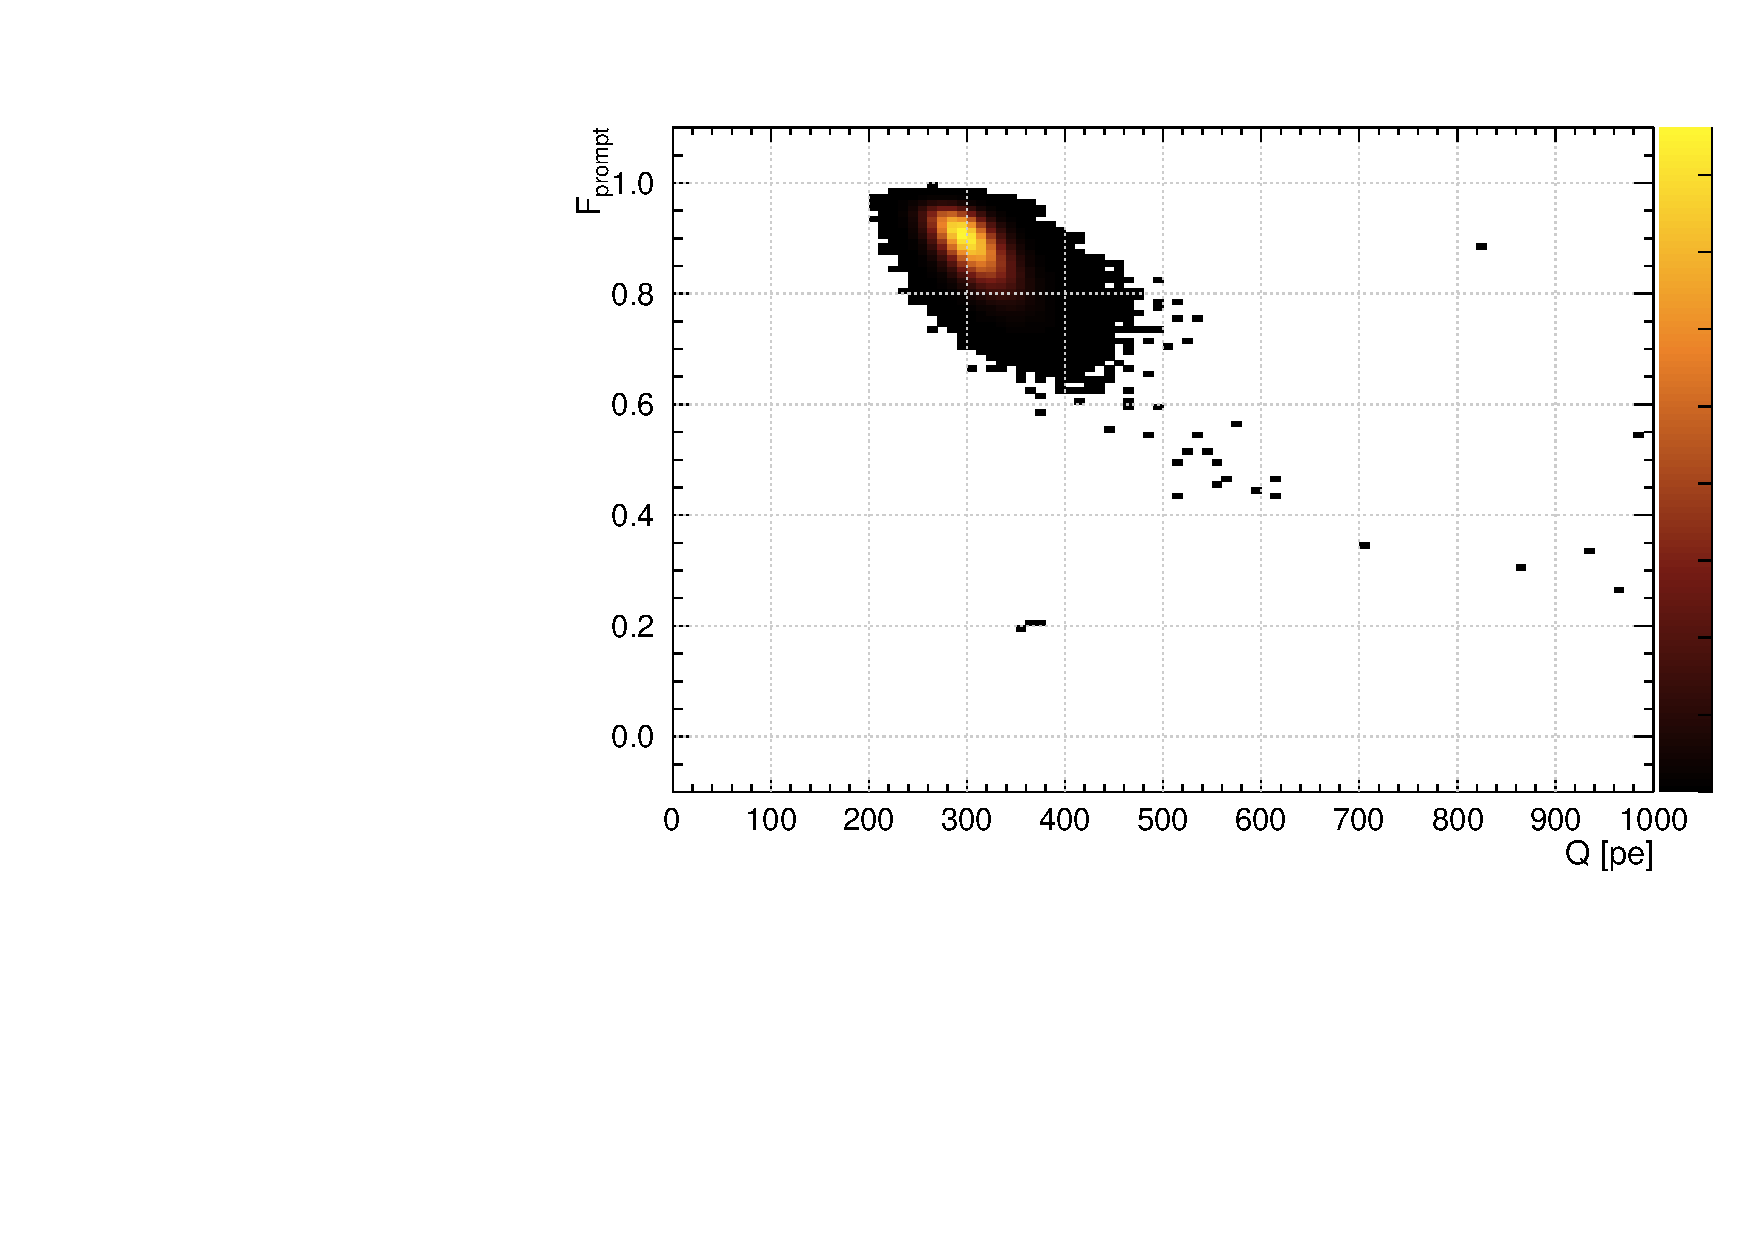
\includegraphics[width=\textwidth]{results/fprompt_015831}
        %\caption{A tiger}
        \label{Fig:fprompt15831}
    \end{subfigure}
    \caption{\textbf{Left:} Typical \gls{aarf} \gls{dtm} waveform for an intensity of 1870. \textbf{Right:} \gls{fprompt} against number of photo electrons recorded per event at an \gls{aarf} intensity of 1870}
    \label{Fig:wf_Fprompt_high}
\end{figure}
\clearpage

%
%\begin{figure}
%\centering
%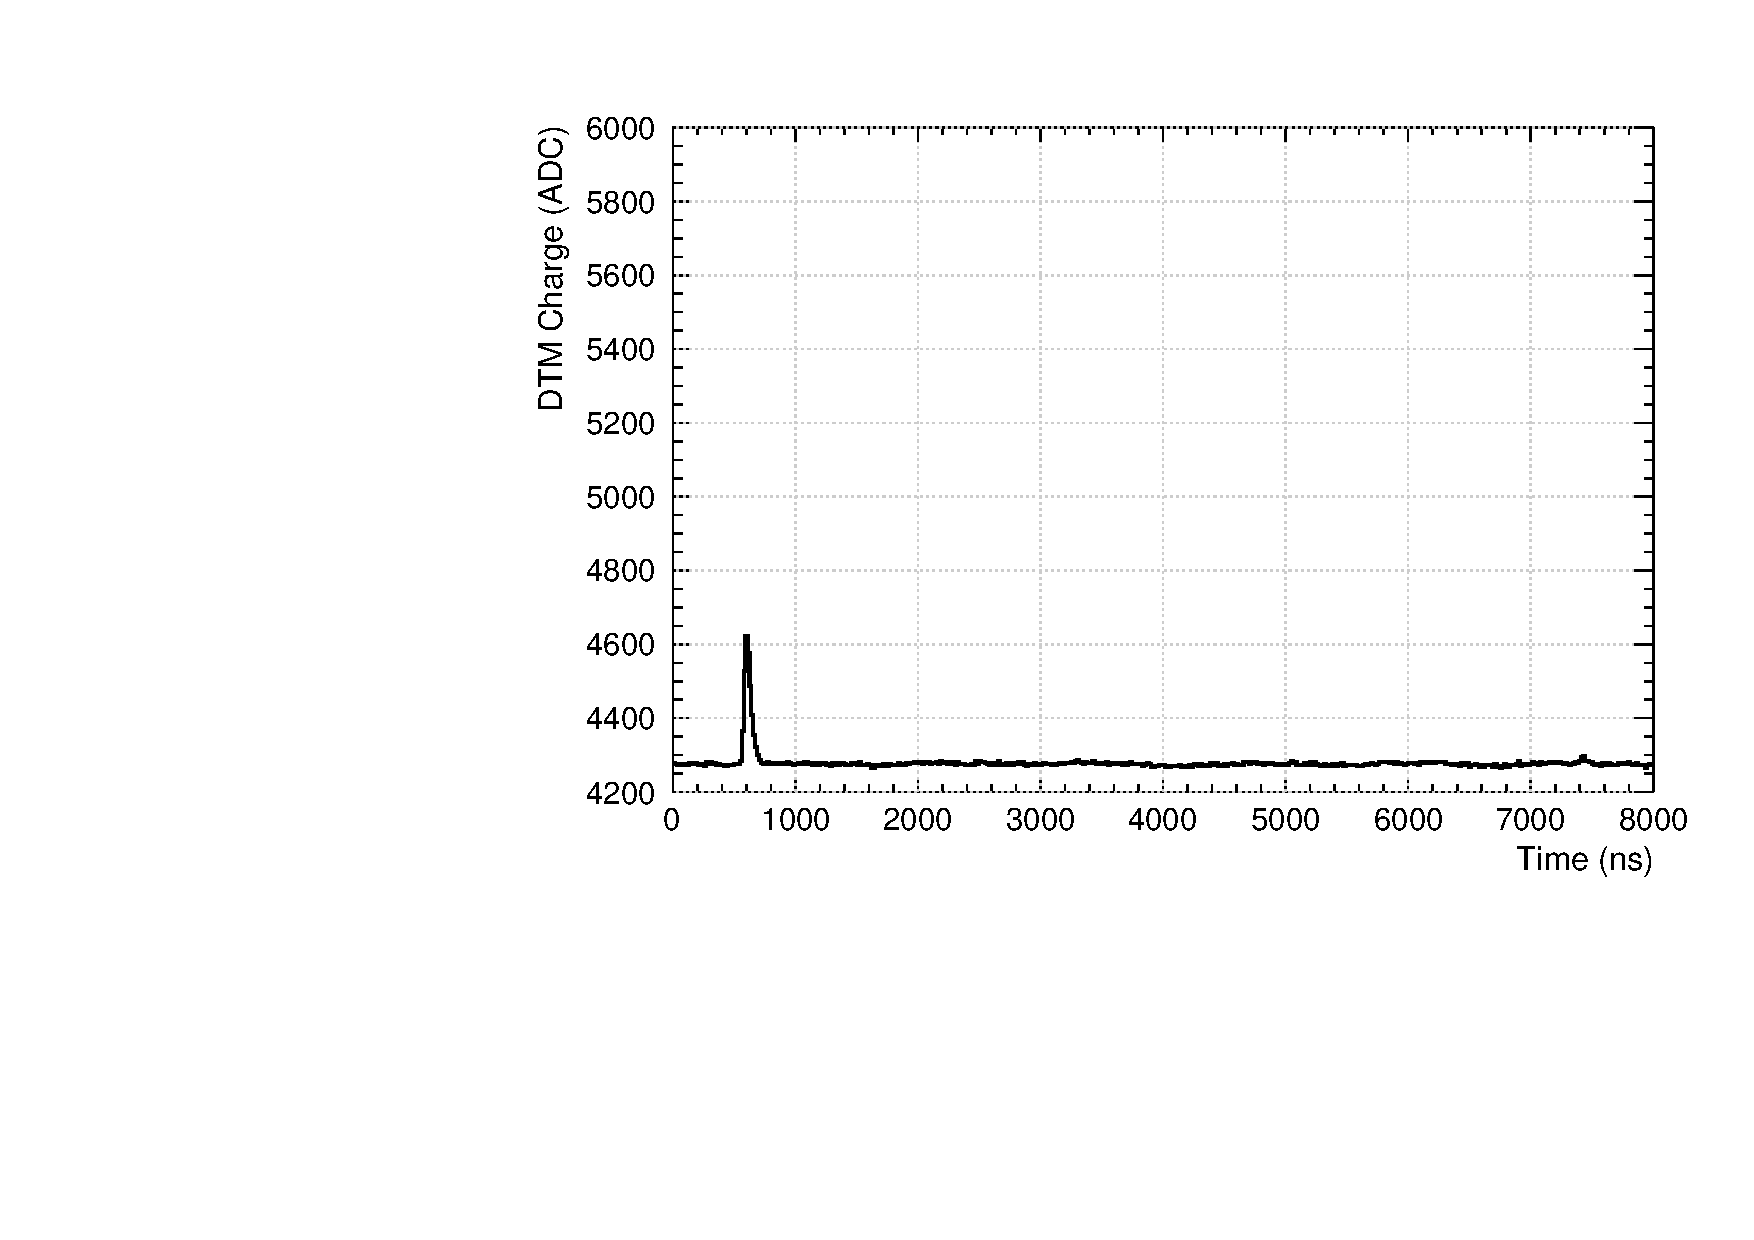
\includegraphics[width=.8\textwidth]{results/dtmWF_15826_1306}
%\caption{Typical \gls{aarf} \gls{dtm} waveform for an intensity of 1270.}
%\label{Fig:wfShort}
%\end{figure}
%
%\begin{figure}
%\centering
%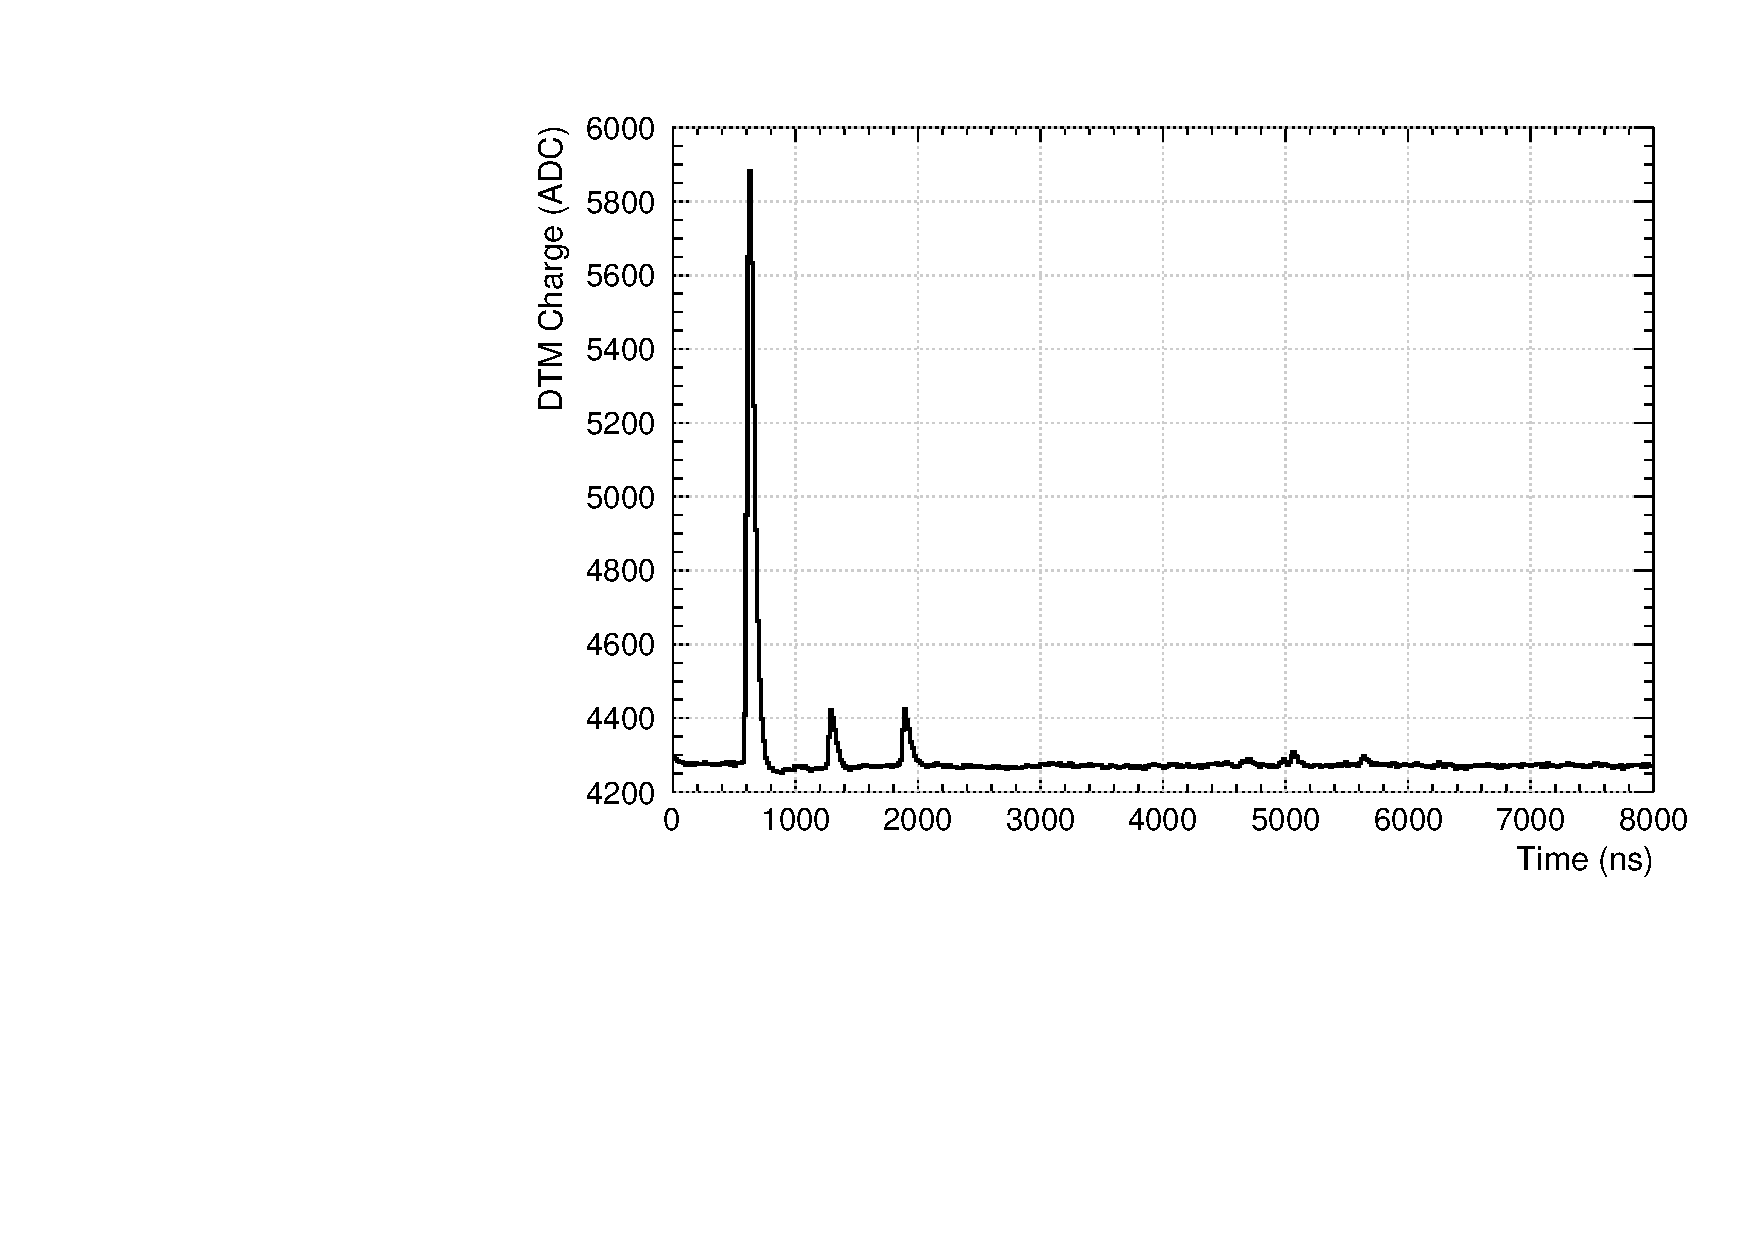
\includegraphics[width=.8\textwidth]{results/dtmWF_15828_405}
%\caption{Typical \gls{aarf} \gls{dtm} waveform for an intensity of 1530.}
%\label{Fig:wfMedium}
%\end{figure}
%
%
%\begin{figure}
%\centering
%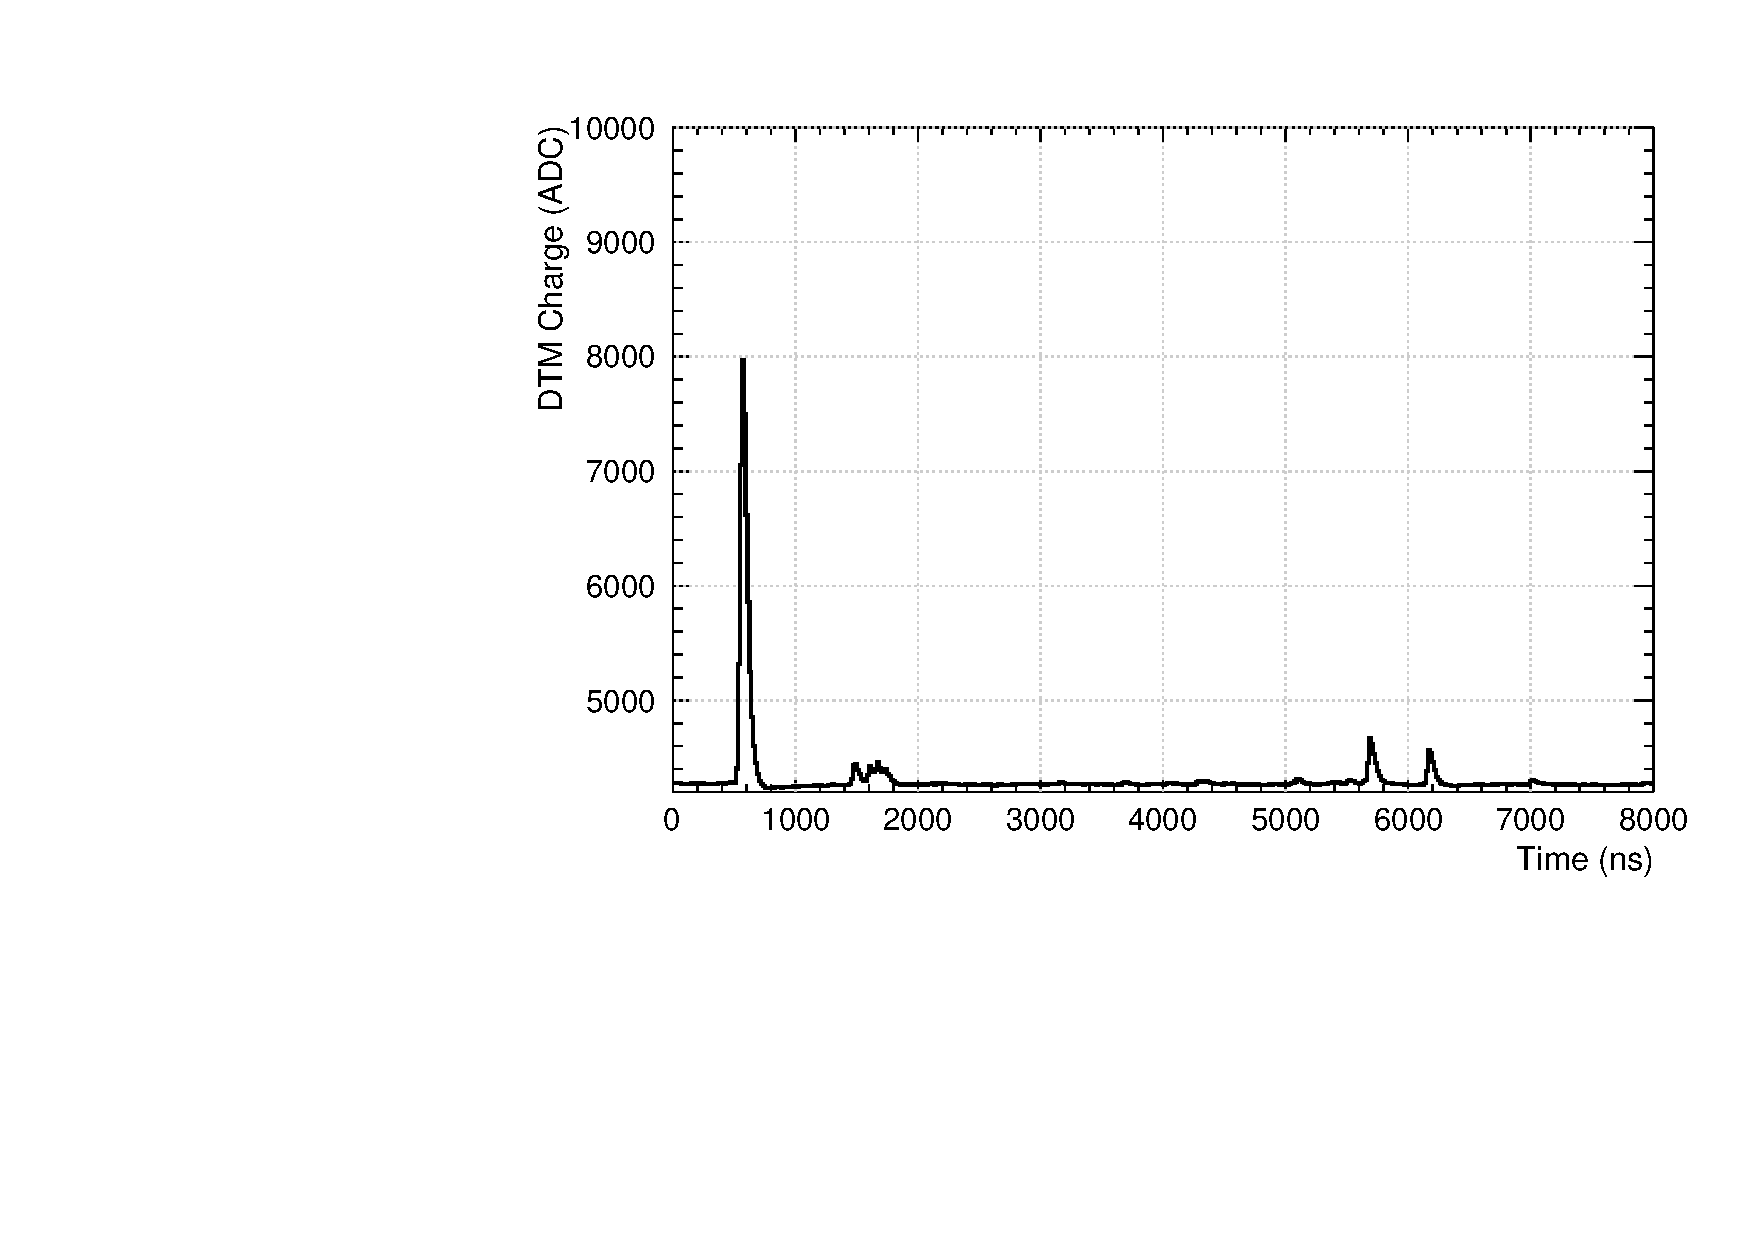
\includegraphics[width=.8\textwidth]{results/dtmWF_15831_718}
%\caption{Typical \gls{aarf} \gls{dtm} waveform for an intensity of 1870.}
%\label{Fig:wfHigh}
%\end{figure}

\begin{figure}
\centering
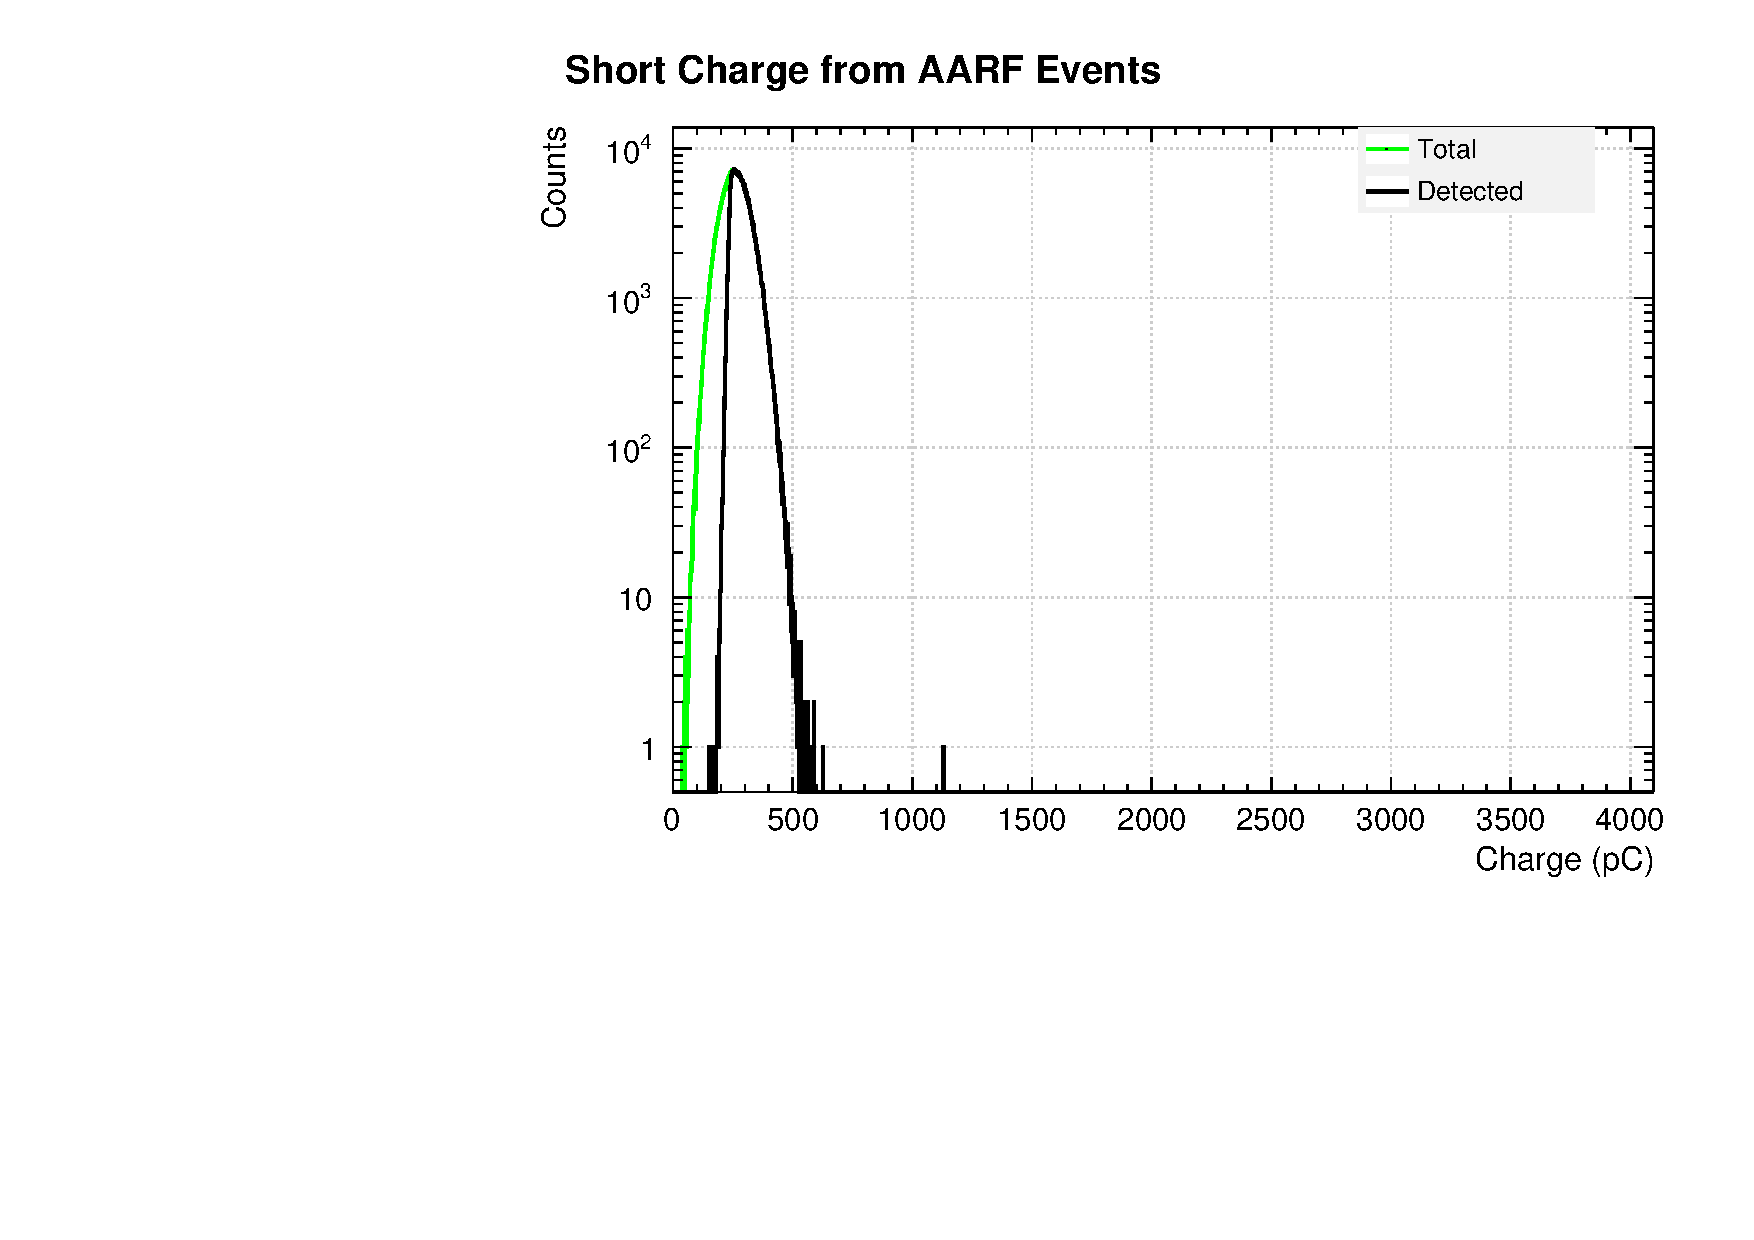
\includegraphics[width=.85\textwidth]{results/chargeHists_dtmThres_1400}
\caption{Histograms of the total light injection events (green) and the events recorded by the trigger (black) for a \gls{dtm} threshold of 1400 ADC}
\label{Fig:effHists1400}
\end{figure}

\begin{figure}
\centering
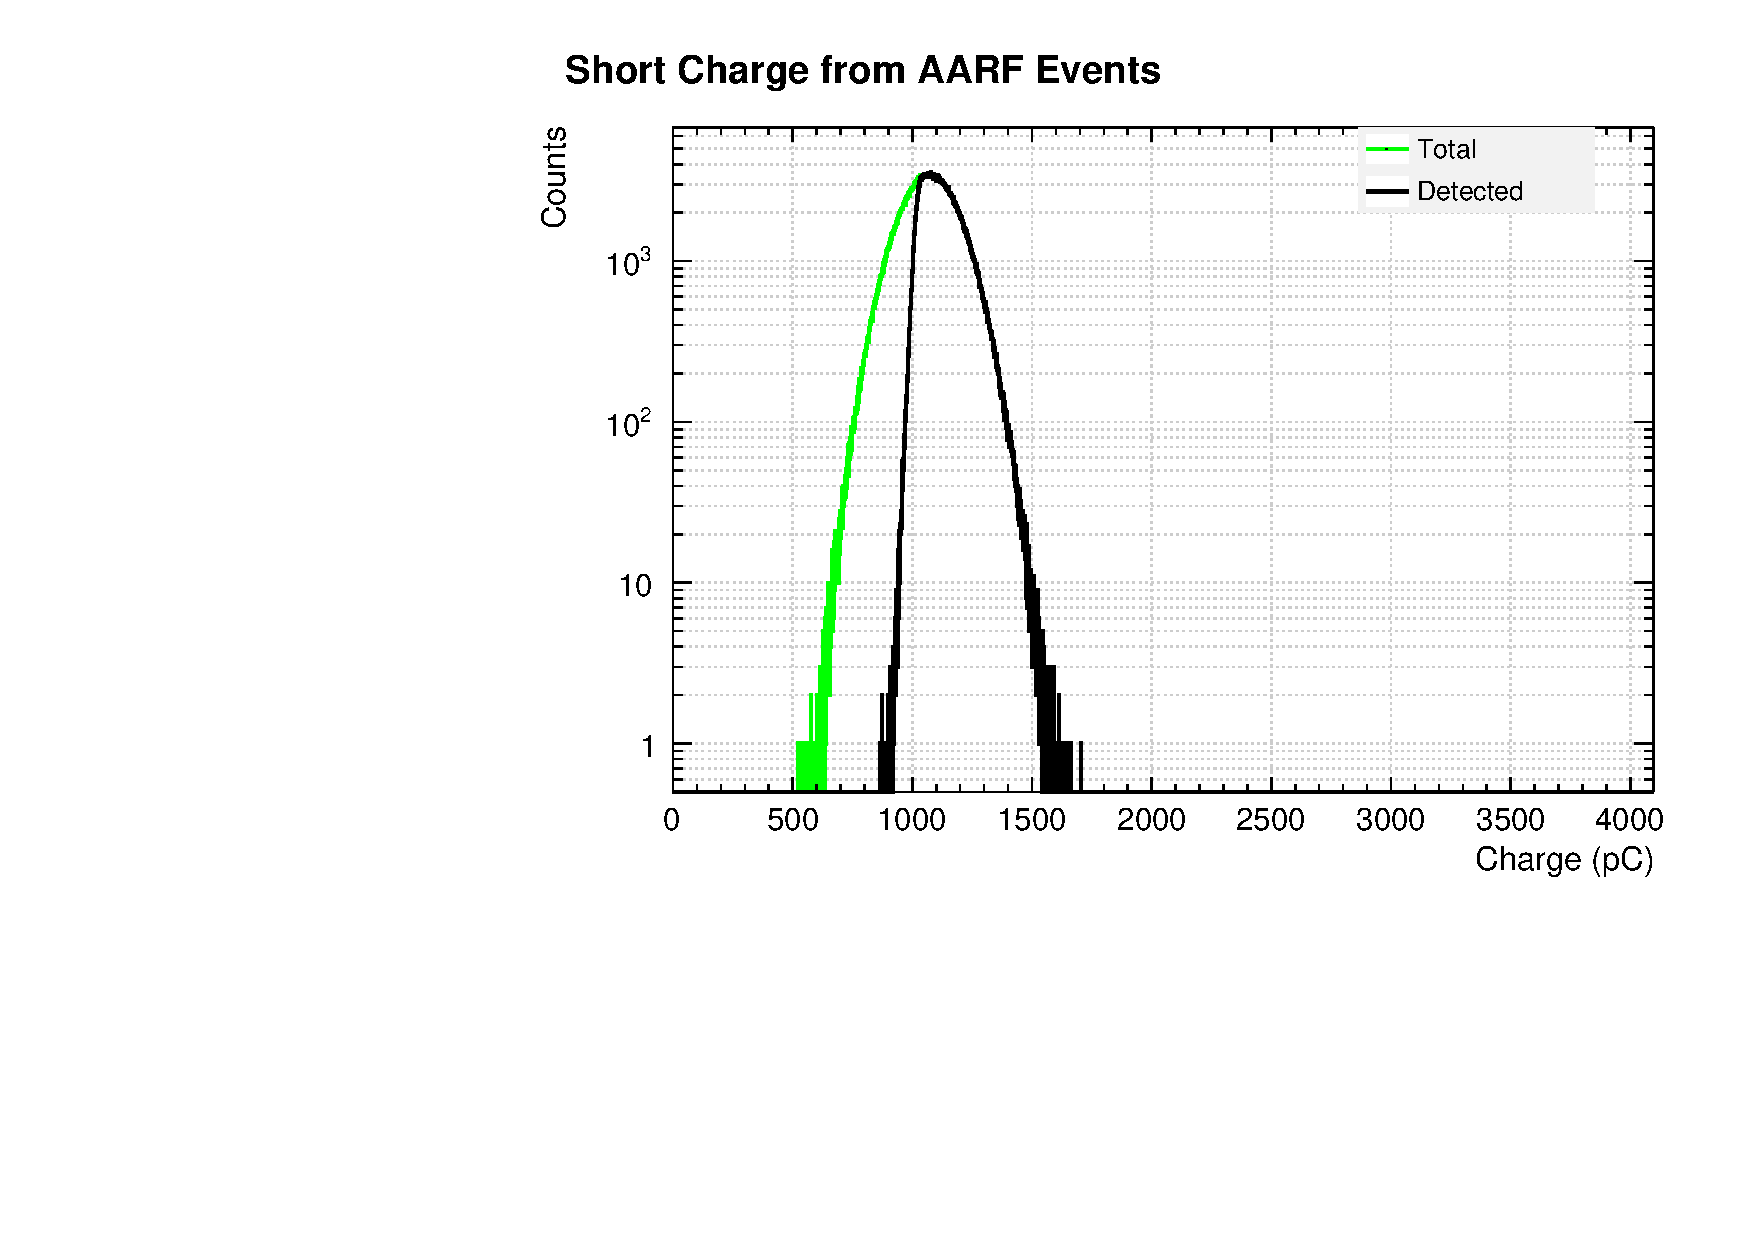
\includegraphics[width=.85\textwidth]{results/chargeHists_dtmThres_6000}
\caption{Histograms of the total light injection events (green) and the events recorded by the trigger (black) for a \gls{dtm} threshold of 6000 ADC}
\label{Fig:effHists6000}
\end{figure}

\begin{figure}
\centering
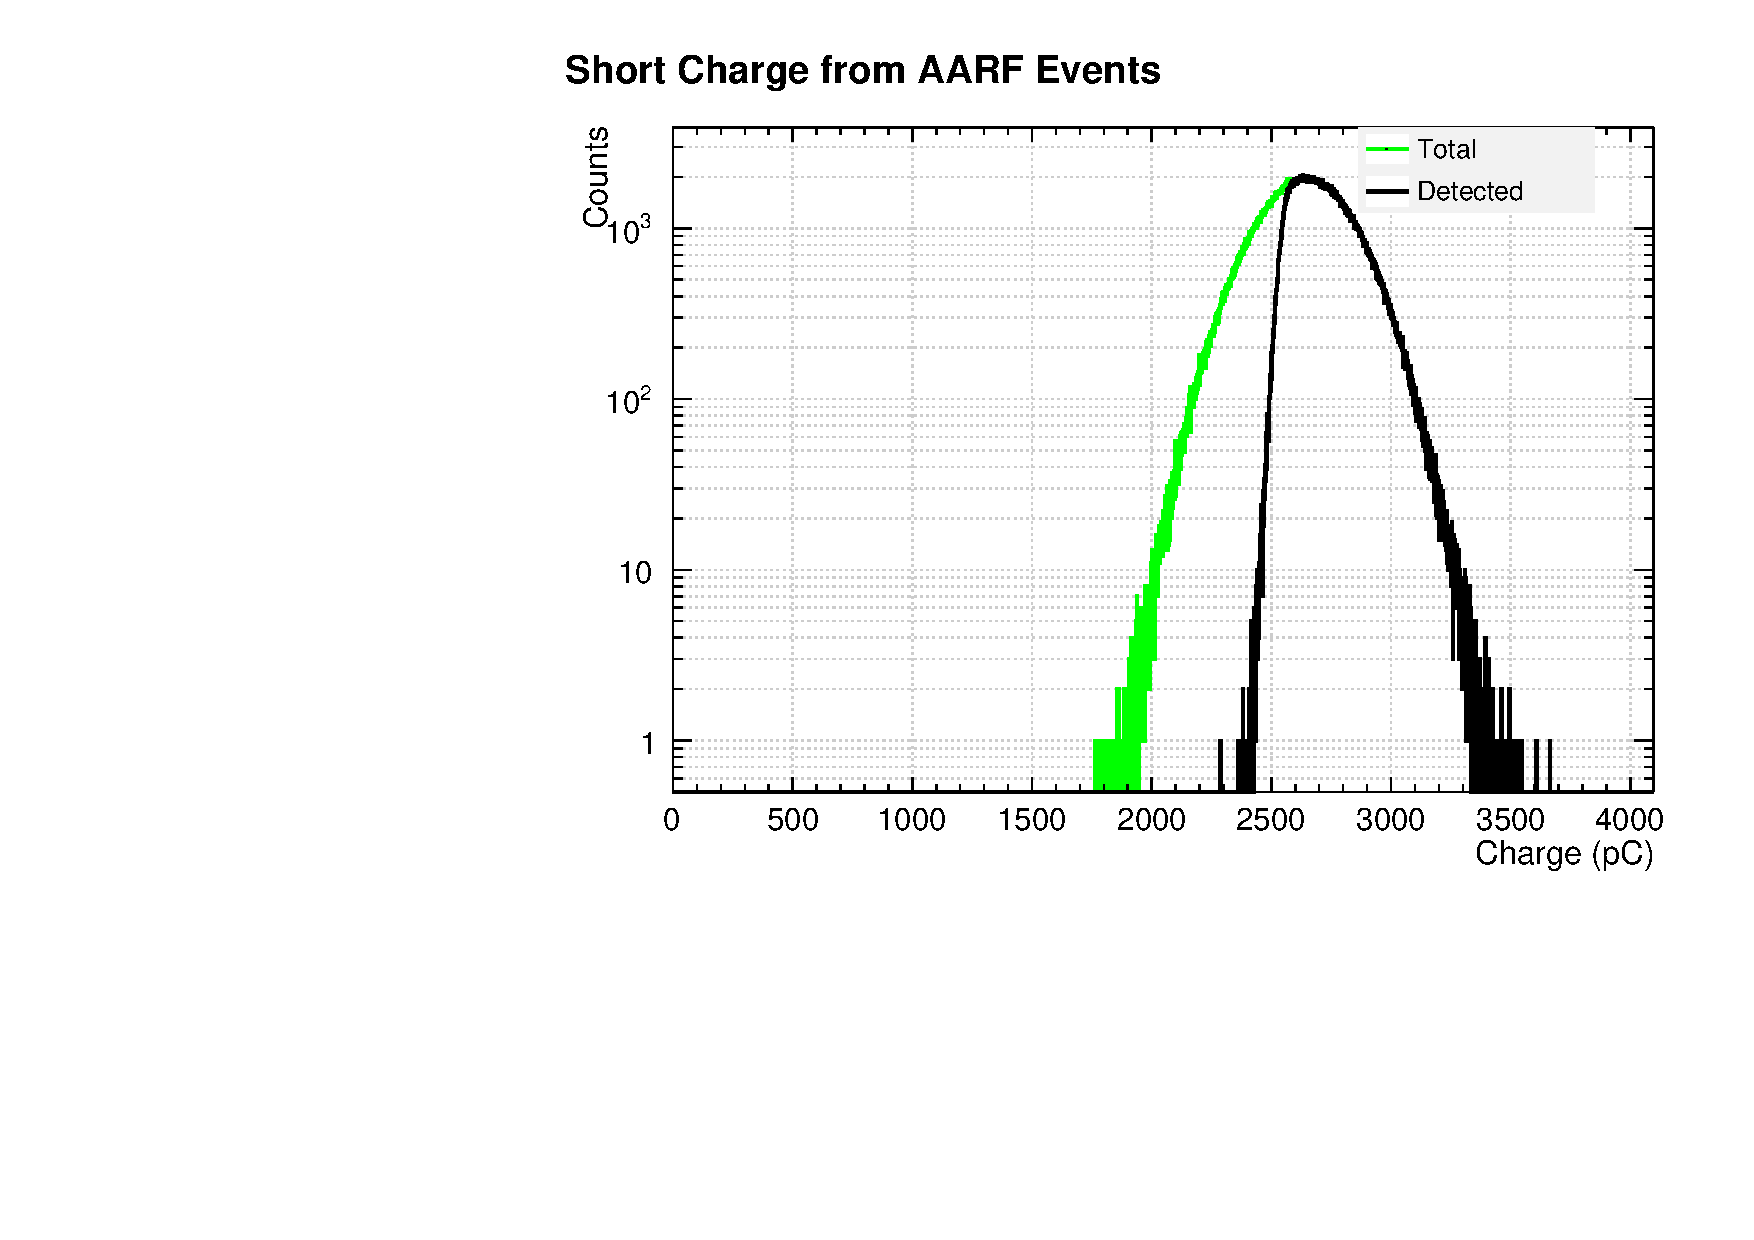
\includegraphics[width=.85\textwidth]{results/chargeHists_dtmThres_15000}
\caption{Histograms of the total light injection events (green) and the events recorded by the trigger (black) for a \gls{dtm} threshold of 15000 ADC}
\label{Fig:effHists15000}
\end{figure}


\clearpage
\section{Error Analysis and Erf Fitting}
The quantity of interest here is the efficiency that an event is recorded by the \gls{dtm} given the value of the V1720 digitizers. Following the work done by Paterno (2004) \cite{paterno2004calculatingErrors}, the uncertainty calculation for the data selection is derived from the application of Bayes's theorem.

\subsection{Bayesian Errors}
For a total of $N$ events in a sample passing a data cut, a probability of selection $\epsilon$, and relevant prior information $I$, the probability that $k$ events are selected is given by the binomial distribution:

\begin{equation}
P(k|\epsilon,N,I) = \frac{N!}{k!(N-k)!} \epsilon^k (1-\epsilon)^{N-k}
\label{Eq:binomial}
\end{equation}
Here we are interested in finding the value of $\epsilon$ from $k,I, \&N$ which are known values. By applying Bayes's theorem to the binomial distribution, the probability that the true selection probability is between $\epsilon$ and $\epsilon$ + d$\epsilon$ ($P(\epsilon|k,N,I)$) can be determined:

\begin{equation}
P(\epsilon|k,N,I) = \frac{P(k|\epsilon,N,I) P(\epsilon,N,I)}{Z}.
\label{Eq:Bayes}
\end{equation}
Here $Z$ is a normalization constant defined as:
\begin{equation}
Z = \frac{N!}{k!(N-k)!} \int_{0}^{1}\epsilon^k (1-\epsilon)^{N-k} d \epsilon.
\label{Eq:baysNormalConst}
\end{equation}
Applying the definition of the beta function:
\begin{equation}
B(x,y) = \int_{0}^{1}t^{x-1} (1-t)^{y-1} dt = \frac{\Gamma(N+2)}{\Gamma(k+1) \Gamma(N-k+1)},
\label{Eq:betaFunc}
\end{equation}
Applying the Beta function to Eq. \eqref{Eq:baysNormalConst}, a solution to Eq. \eqref{Eq:Bayes} can be expressed as:
\begin{equation}
P(\epsilon|k,N,I) = \frac{\Gamma(N+2)}{\Gamma(k+1)\Gamma(N-k+1)} \epsilon^k (1-\epsilon)^{N-k}
\label{Eq:BayesWithBeta}
\end{equation}
This formulation will give a most probable value of the selection probability $k/N$, however finding the exact uncertainty is non-trivial.

The probability that $\epsilon$ is in the range $[\alpha, \beta]$ is denoted $\lambda$ and is taken in this study to be one sigma or 68.3$\%$. $\lambda$ is given by:

\begin{equation}
\int_{\alpha}^{\beta}P(\epsilon|k,N,I)d \epsilon = \lambda.
\label{Eq:lambdaEqn}
\end{equation}
Finding the smallest interval $[\alpha, \beta]$ will give the confidence level that $\epsilon$ falls within this range. Minimizing this interval is done through the application of Lagrange multipliers, leading to the simultaneous non-linear equations:

\begin{eqnarray}
G + \rho \alpha^k (1-\alpha)^{N-k} &=& 0\\
G + \rho \beta^k (1-\beta)^{N-k} &=& 0\\
B_{\beta}(k+1,N-k+1) - B_{\alpha}(k+1, N-k+1) &=& \lambda G.
\label{Eq:lagrangeEqns}
\end{eqnarray}
Here G is $\Gamma(k+1)\Gamma(N-k+1/\Gamma(N+2))$, $\rho$ is a Lagrange multiplier and $B_x(u,v)$ is the partial Beta function defined as:
\begin{equation}
B_x(u,v) = \int_{0}^{x}t^{u-1}(1-t)^{v-1}dt.
\label{Eq:partialBeta}
\end{equation}

This error solution, formulated by Paterno (2004) \cite{paterno2004calculatingErrors}, has been included in the \gls{root} data analysis framework with the TEfficiency class \cite{root}.


\subsection{Erf Fitting}
The Gaussian error function (or \gls{erf}) naturally arises as the threshold of a Gaussian selection \cite{Casadei2012SelectionEfficiency}, such as is expected in the \gls{dtm}. The erf is defined as:

\begin{equation}
\text{erf}(x) = \frac{2}{\sqrt{\pi}} \int_{0}^{x} e^{-\tau ^2}d\tau
\label{Eq:erf}
\end{equation}
Assuming there is no significant excess noise, interference, or non-Gaussian behaviour, it is expected that the \gls{dtm} efficiency as a function of the total \gls{v1720} short window charge would be well fit to an \gls{erf}. If an event has a \gls{v1720} short window charge that falls within a turn on region, there is a possibility of being categorized as either of the two energy regions being transitioned between. Characterizing these regions with an \gls{erf} allows for the inclusion of this statistical possibility of being miscategorized by the \gls{dtm}, and a deeper knowledge of the uncertainty. In operation the trigger regions being pre-scaled will have to be chosen is such a way to minimize the possibility of pre-scaling a non-$\beta$ event while not saturating the \gls{daq} with events. This will be done once the rate of $\beta$-decay events in the detector is appreciable as it is being filled with argon.
   
The histograms of the total and detected events for each \gls{aarf} intensity at a given \gls{dtm} threshold are combined to ensure high statistics at the turn-on region of the \gls{dtm} (see Fig. \ref{Fig:effHists1400} -\ref{Fig:effHists15000}). Using the \gls{root} TEfficiency class, these histograms are divided to give the efficiencies shown in Fig. \ref{Fig:effFit1400} -\ref{Fig:effFit15000}. An \gls{erf} function with a mean ($\mu$) and standard deviation ($\sigma$) is fit to the turn on curves as a function of the \gls{v1720} charge ($\epsilon$) given by:


\begin{equation}
f(\epsilon,\mu,\sigma) = \left( \frac{1}{2} \right) \left( 1+\text{erf}\left(\frac{\epsilon-\mu}{\sqrt{2}\sigma}\right)\right)
\label{Eq:fitErf}
\end{equation}


\clearpage
\begin{figure}
\centering
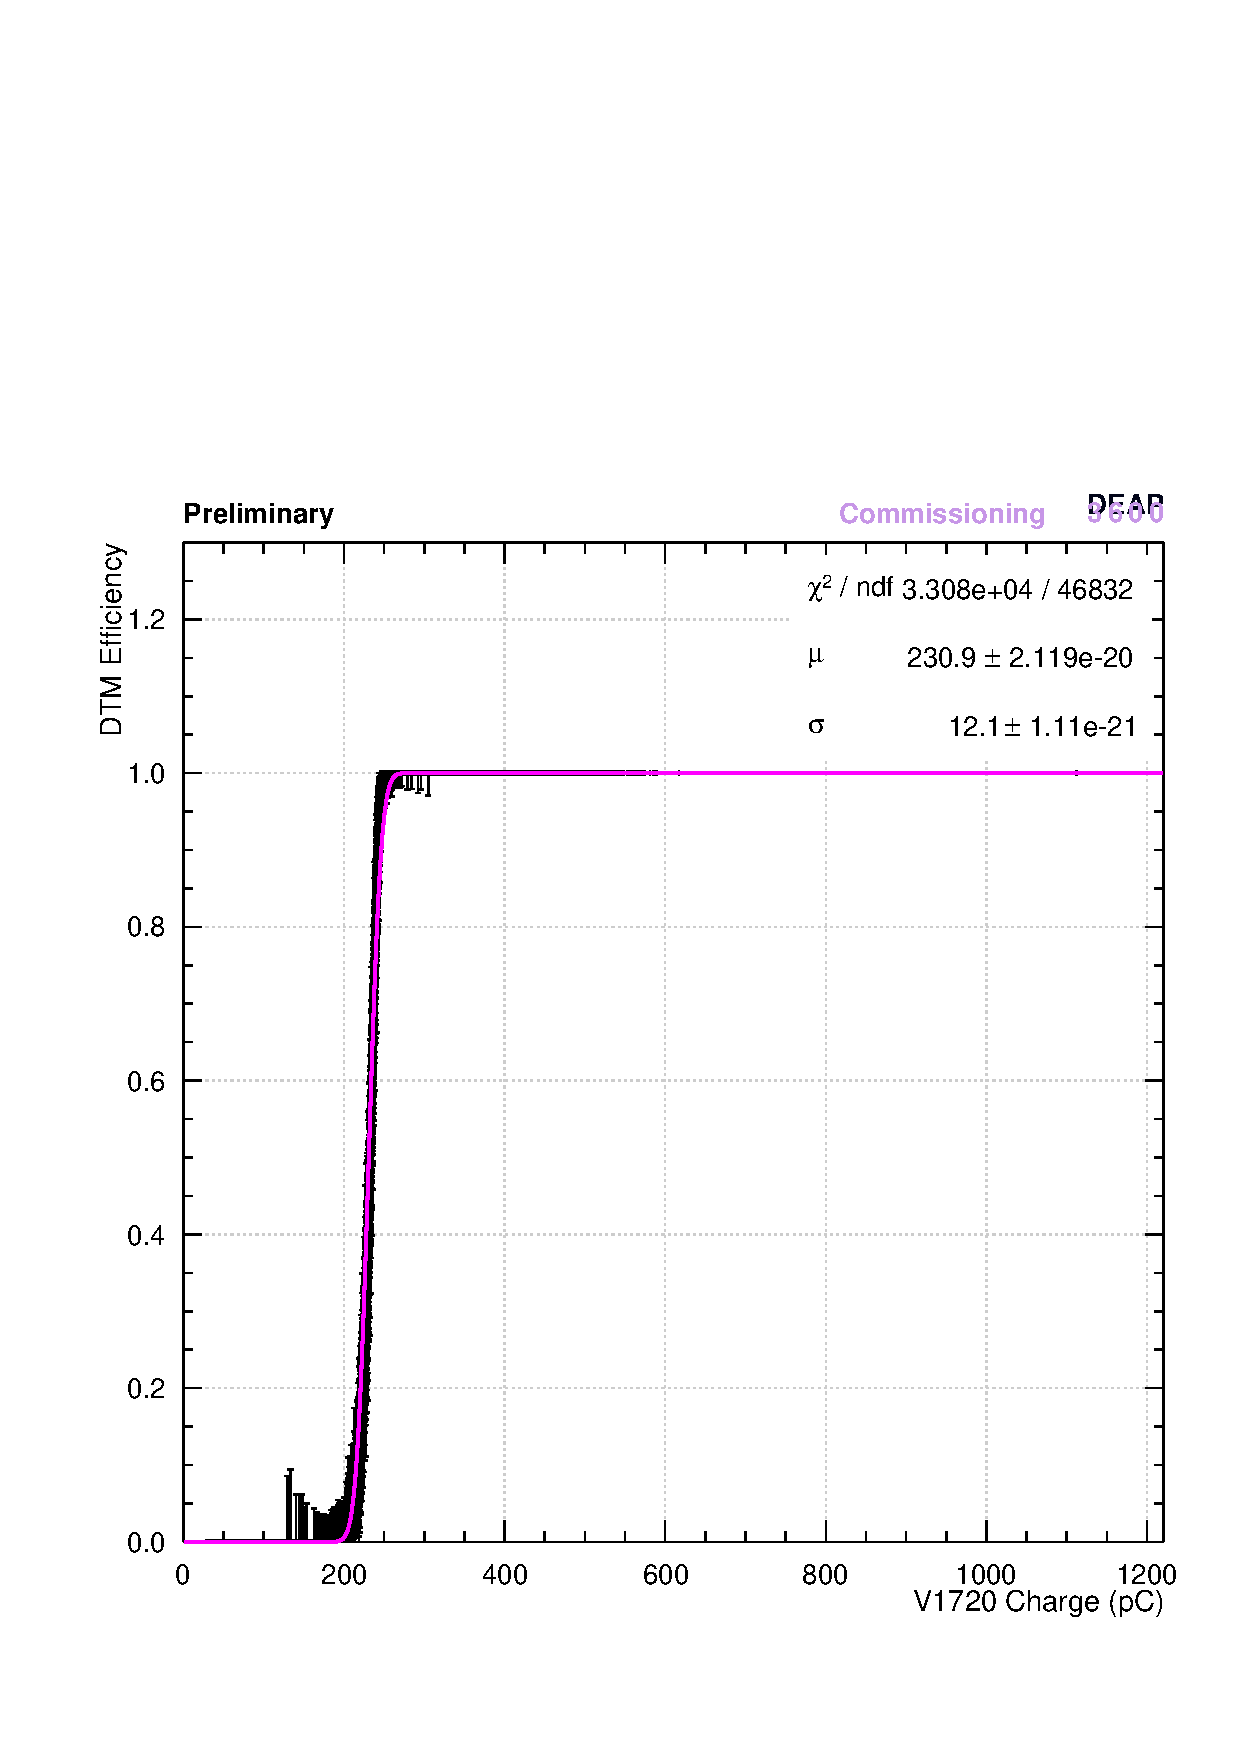
\includegraphics[width=.85\textwidth]{results/effPlot_dtmThres_1400}
\caption{Efficiency of the trigger for a \gls{dtm} threshold of 1400 ADC. The efficiency is taken from the histograms given in Fig. \ref{Fig:effHists1400} and is fit to a Gaussian error function (Eq. \eqref{Eq:fitErf}).}
\label{Fig:effFit1400}
\end{figure}
\clearpage
\begin{figure}
\centering
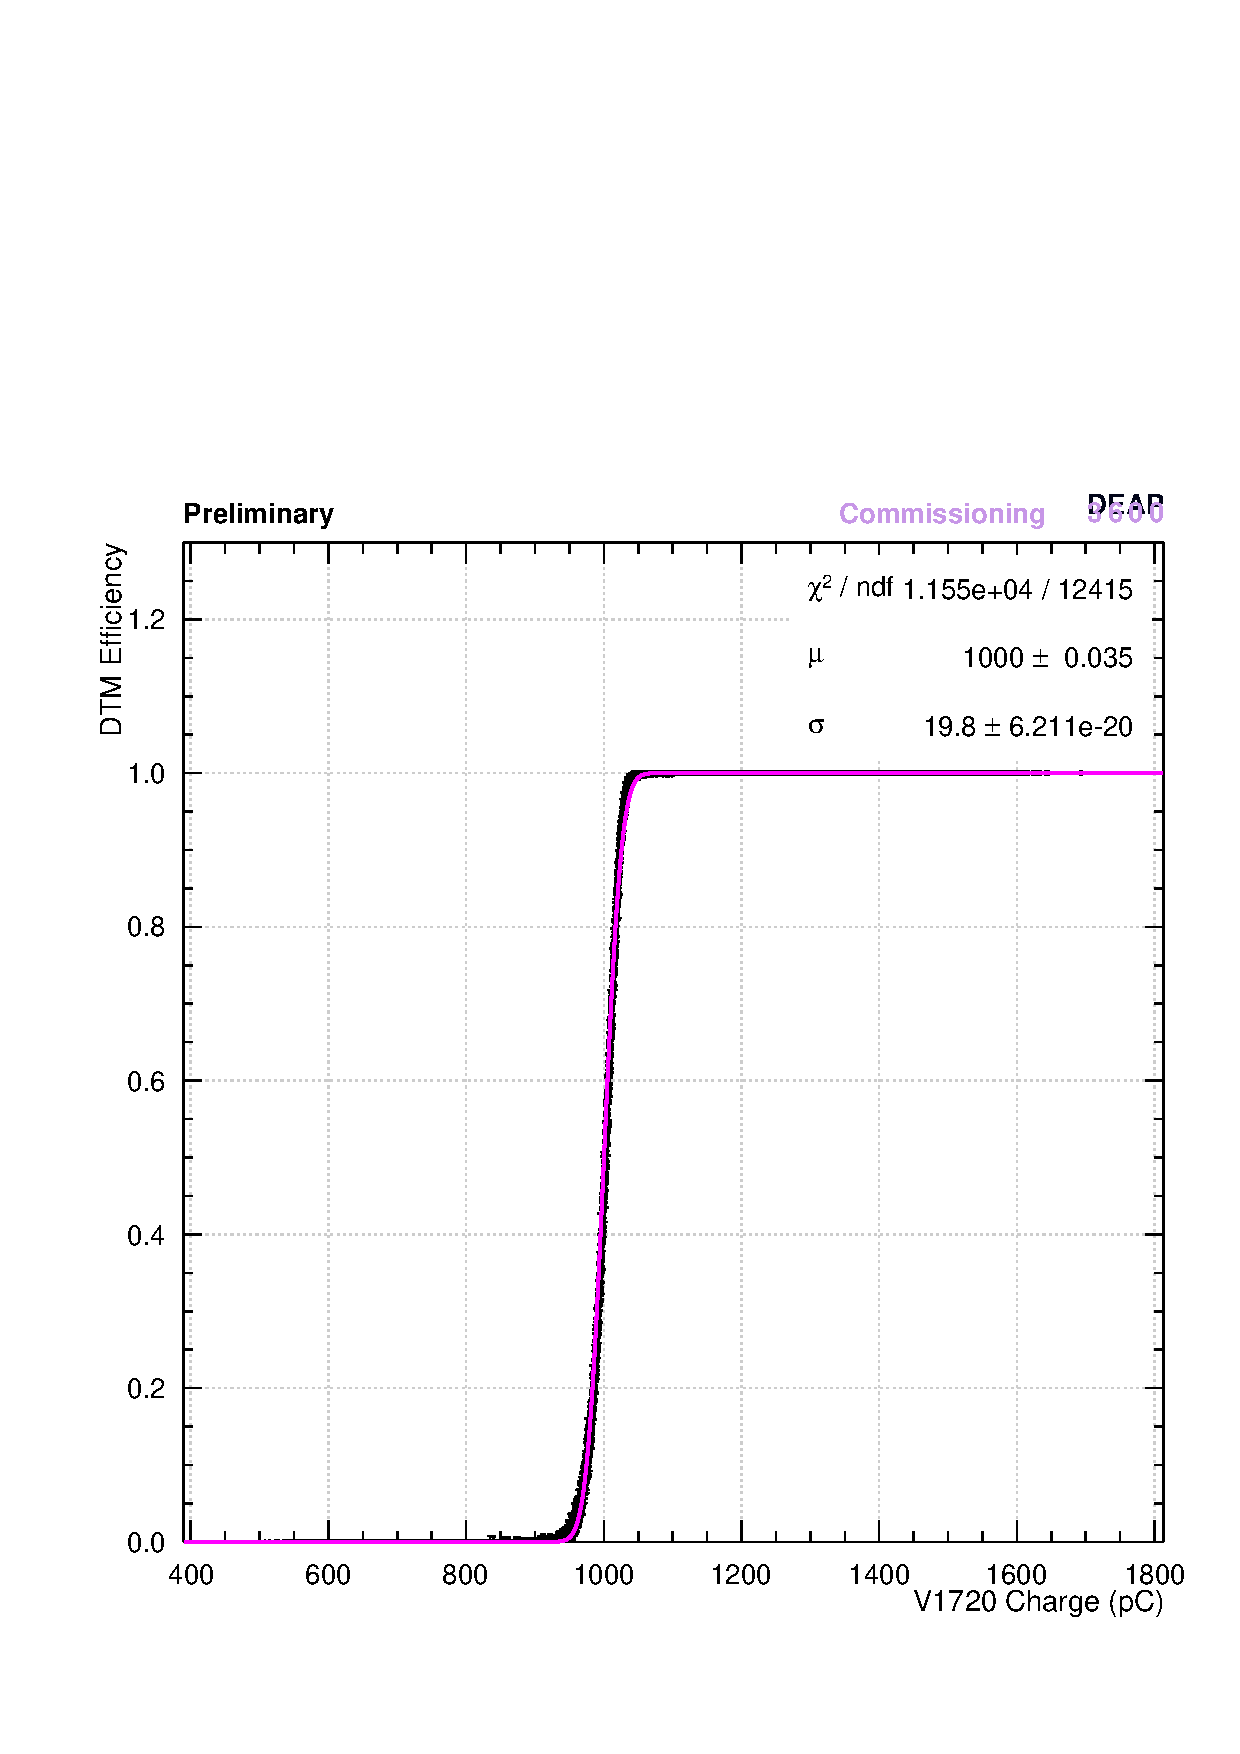
\includegraphics[width=.85\textwidth]{results/effPlot_dtmThres_6000}
\caption{Efficiency of the trigger for a \gls{dtm} threshold of 6000 ADC. The efficiency is taken from the histograms given in Fig. \ref{Fig:effHists6000} and is fit to a Gaussian error function (Eq. \eqref{Eq:fitErf}).}
\label{Fig:effFit6000}
\end{figure}
\clearpage
\begin{figure}
\centering
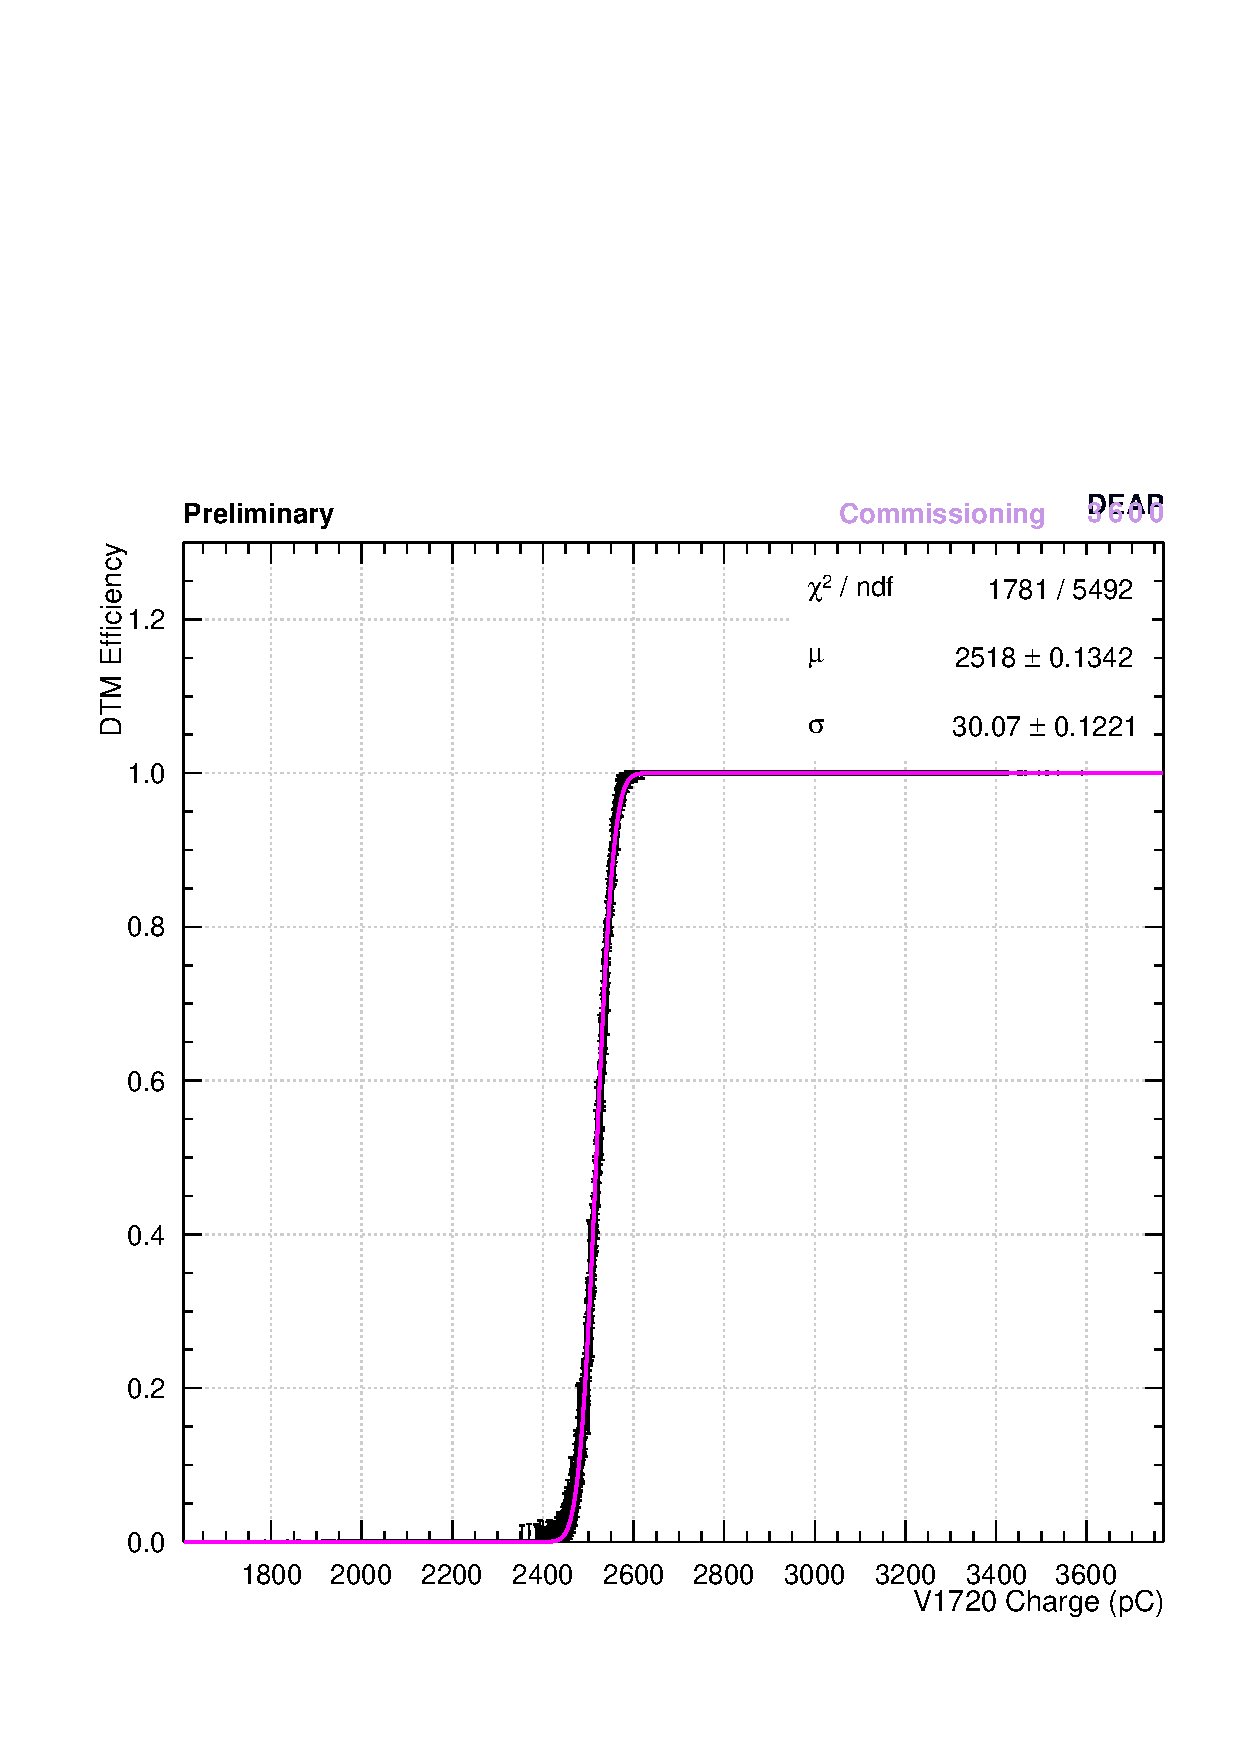
\includegraphics[width=.85\textwidth]{results/effPlot_dtmThres_15000}
\caption{Efficiency of the trigger for a \gls{dtm} threshold of 15000 ADC. The efficiency is taken from the histograms given in Fig. \ref{Fig:effHists15000} and is fit to a Gaussian error function (Eq. \eqref{Eq:fitErf}).}
\label{Fig:effFit15000}
\end{figure}
\clearpage
The spread in the trigger efficiency is due to the differences in charge calculation between the \gls{dtm} and the \gls{v1720}s. The \gls{dtm} receives the analog sum of the \gls{scb} inputs (the \gls{asum}s) and integrates the digital sum of them (the \gls{ass}) over a short time window centred at an events pulse peak. The analog \gls{asum}s receive the entire signal from the \gls{pmt}s, the difference in which can be seen in the charge comparison histograms for recorded events shown in Fig. \ref{Fig:charge1400}-\ref{Fig:charge15000} for each of the different thresholds; note the clean cut off in the \gls{dtm} charge at the \gls{dtm} threshold value.

\clearpage
\begin{figure}
\centering
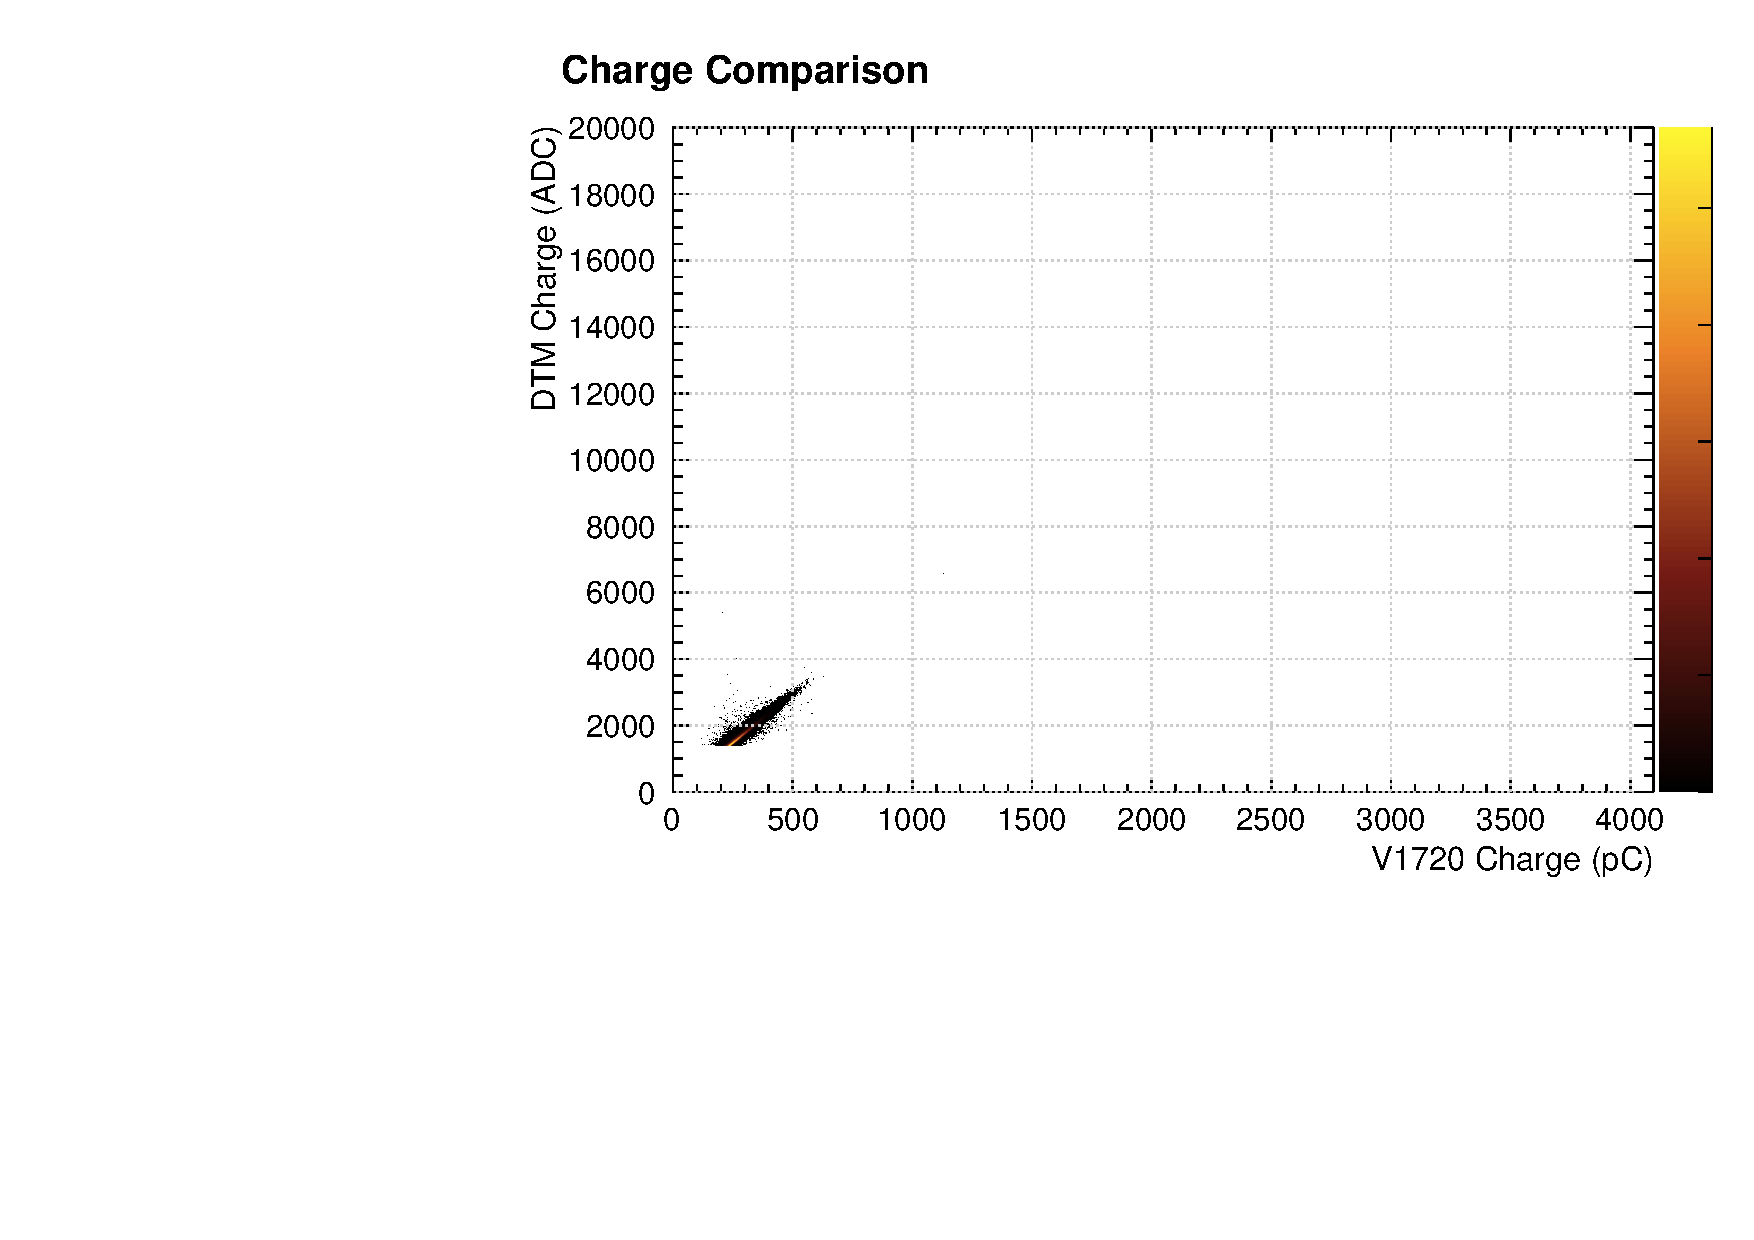
\includegraphics[height=.3\paperheight]{results/realChargeComp_dtmThres_1400}
\caption{Charge histogram comparing the charge recorded by the \gls{dtm} and by the \gls{v1720}s for a threshold of 1400 ADC. Although quite a tight charge relation, the spread in value introduces an uncertainty causing the Gaussian shape that is seen in the efficiency analysis}
\label{Fig:charge1400}
\end{figure}
\begin{figure}
\centering
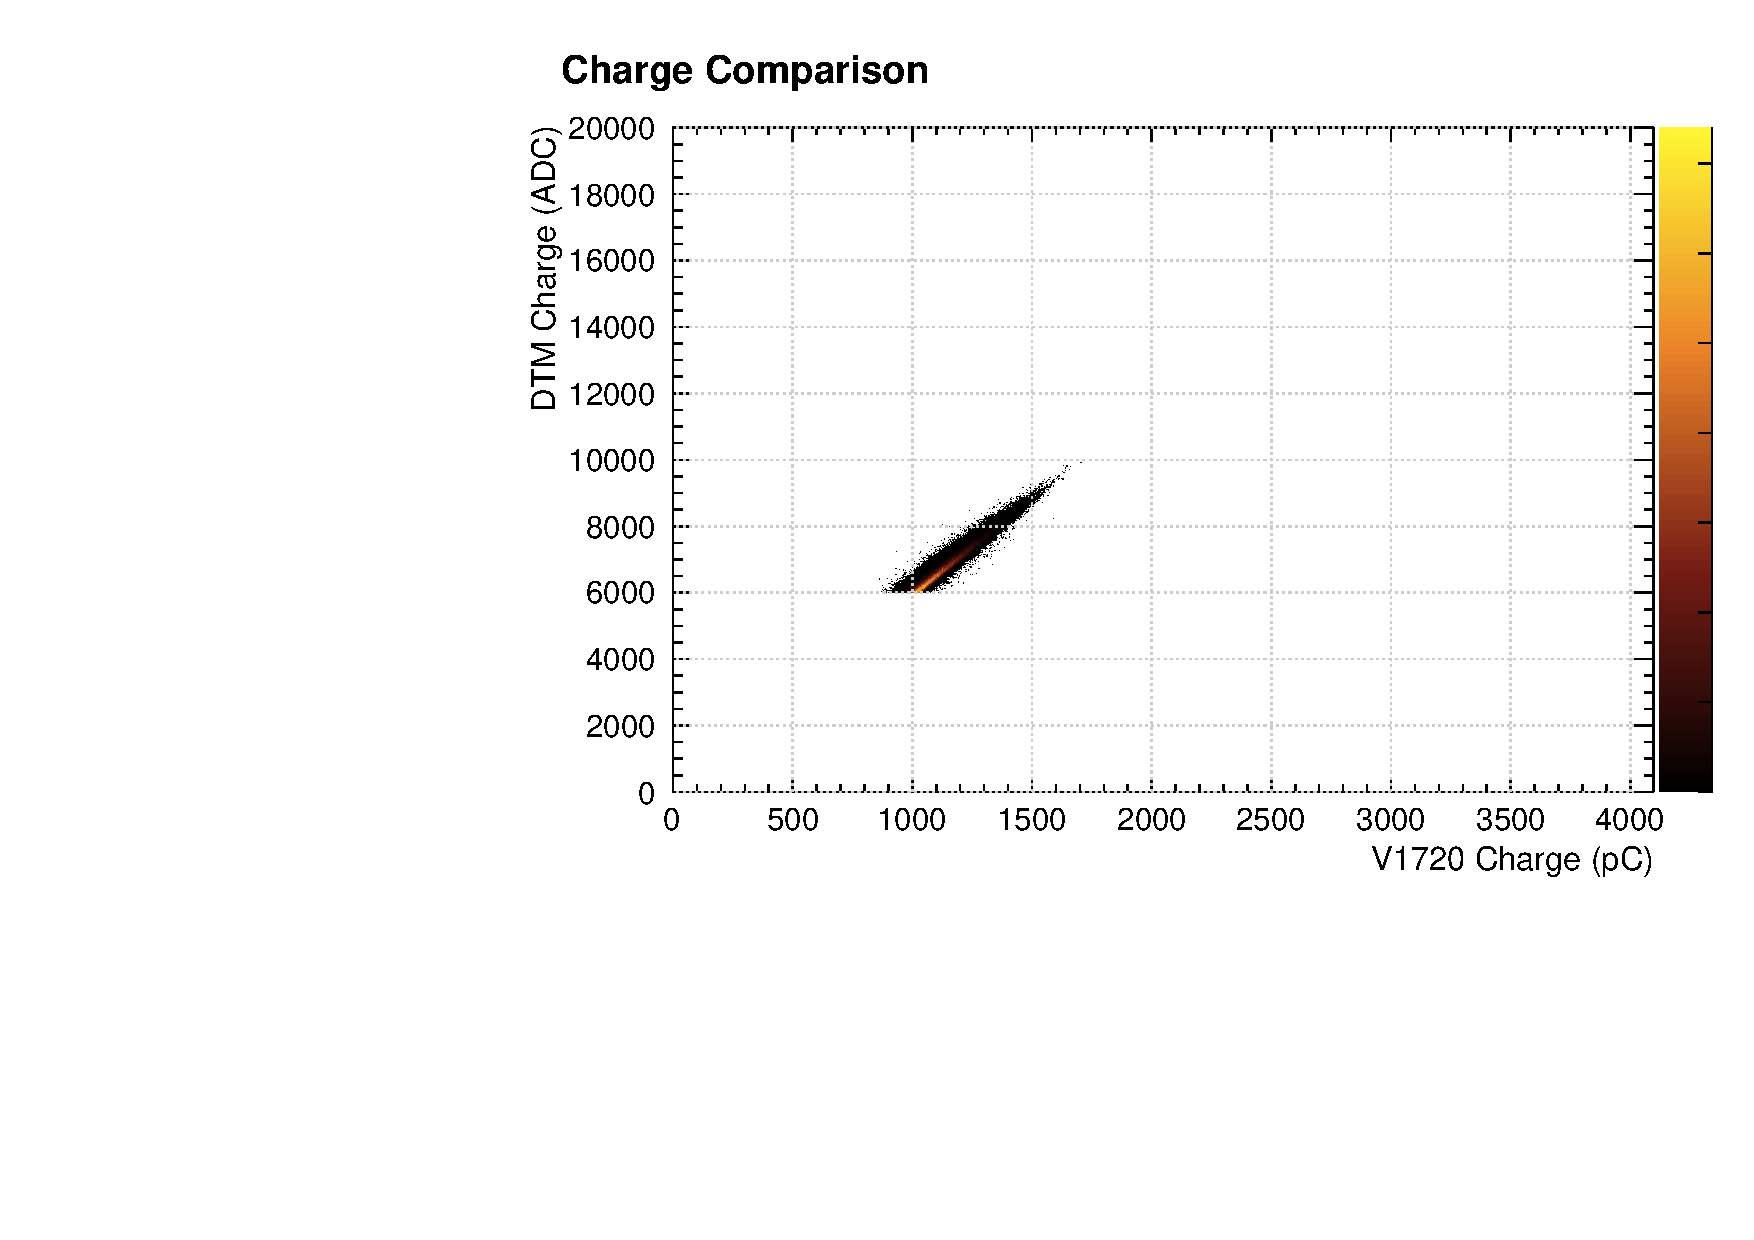
\includegraphics[height=.3\paperheight]{results/realChargeComp_dtmThres_6000}
\caption{Charge histogram comparing the charge recorded by the \gls{dtm} and by the \gls{v1720}s for a threshold of 6000 ADC. Although quite a tight charge relation, the spread in value introduces an uncertainty causing the Gaussian shape that is seen in the efficiency analysis}
\label{Fig:charge6000}
\end{figure}
\begin{figure}
\centering
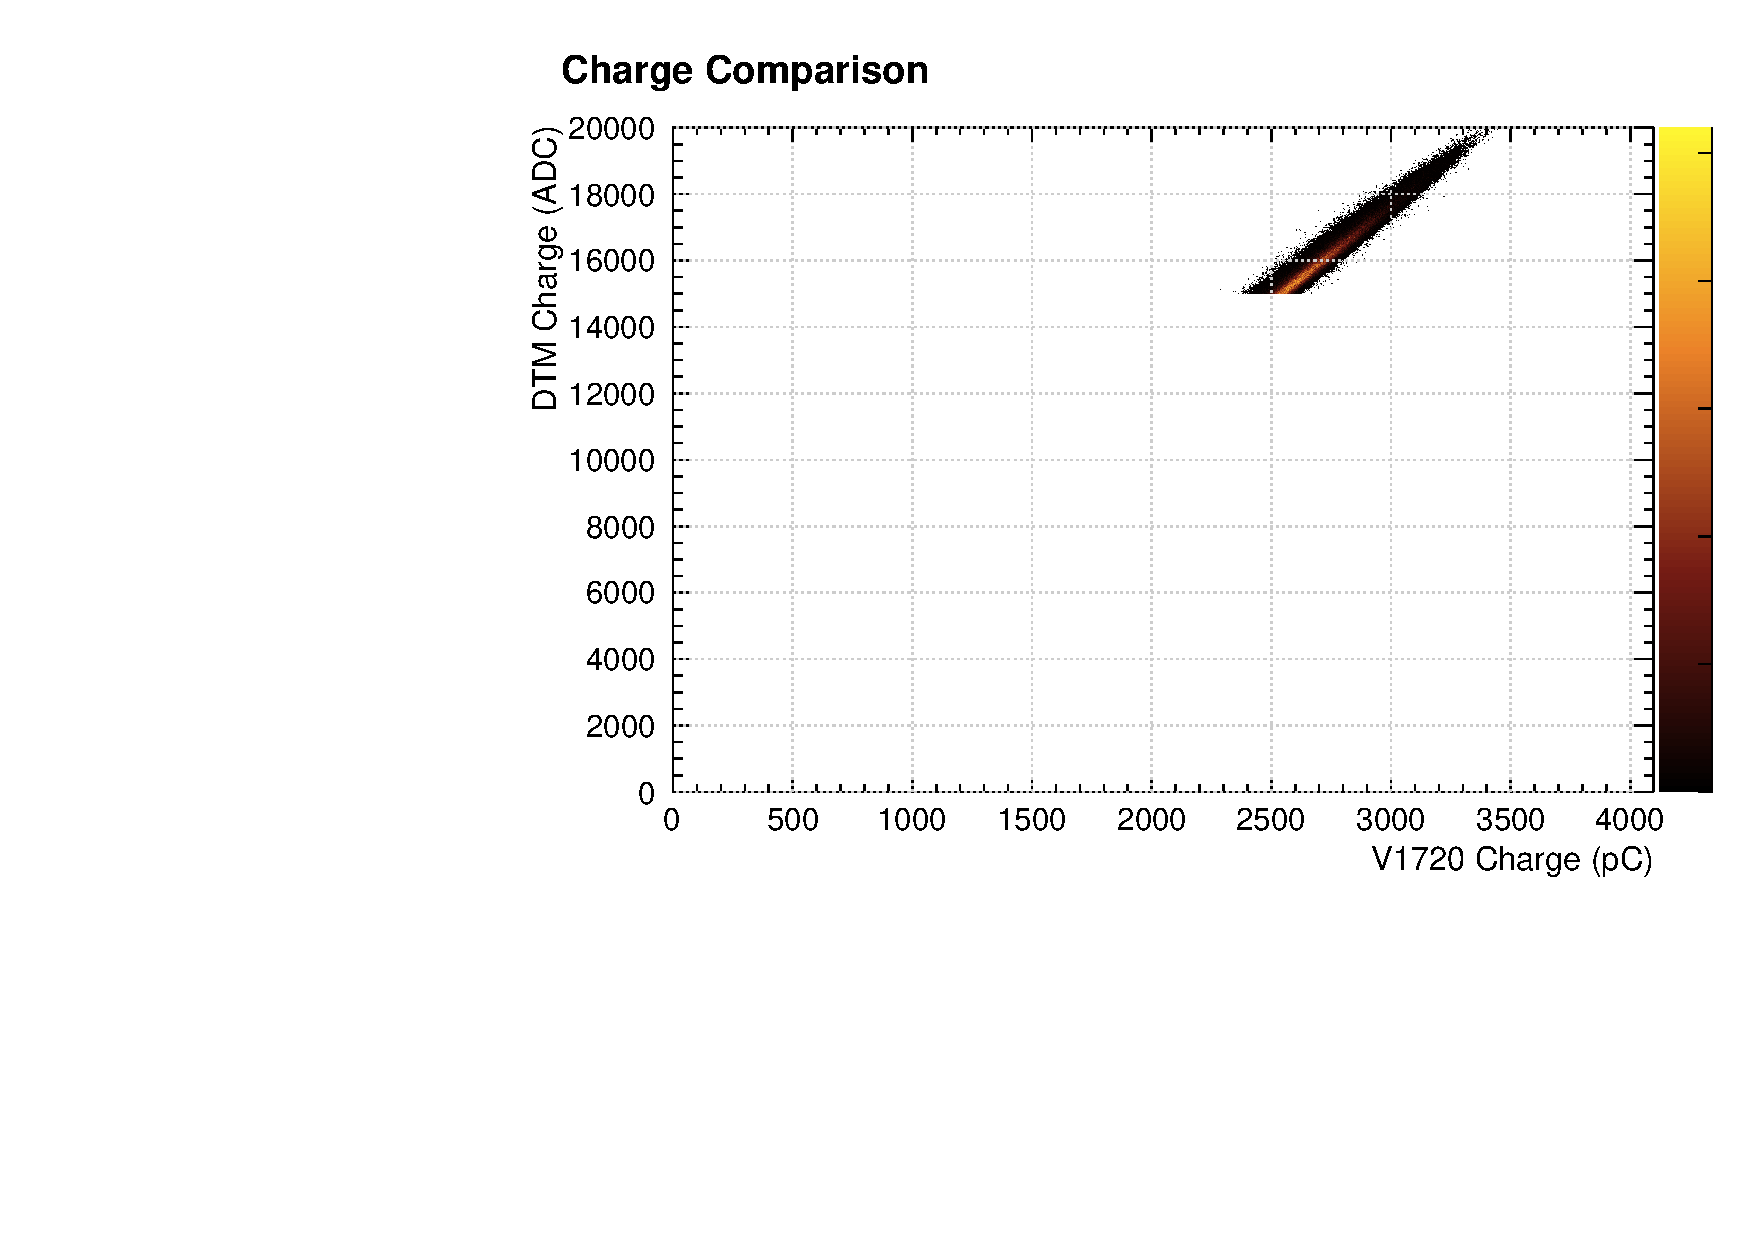
\includegraphics[height=.3\paperheight]{results/realChargeComp_dtmThres_15000}
\caption{Charge histogram comparing the charge recorded by the \gls{dtm} and by the \gls{v1720}s for a threshold of 15000 ADC. Although quite a tight charge relation, the spread in value introduces an uncertainty causing the Gaussian shape that is seen in the efficiency analysis}
\label{Fig:charge15000}
\end{figure}
\clearpage


\begin{table}[h]
\centering
\caption{Fit parameters to the charges recorded for each run type.}
\vspace{0.2cm}
\begin{tabular}{c	c	c	c}
\hline
\hline
\textbf{DTM Threshold}&		\textbf{Run}&		\textbf{$\mu$ (pC)}&		\textbf{$\sigma$ (pC)}\\
\textbf{(ADC)}&		&		&		\\

\hline
1400&	304&	230.9 $\pm$ 2.1e-20& 	12.1$\pm$1.1e-21\\		
6000&	305&	1000 $\pm$ 0.035& 	19.8$\pm$6.2e-20\\
15000&	306&	2518 $\pm$ 0.13& 	30.07$\pm$0.12\\
\hline
\hline
\end{tabular}
\label{Table:erfFitVals}
\end{table}
%
%\section{Charge Calibration}
%\label{sec:ChargeCalib}
%LOOK AT CHARGES, MAKE HISTOGRAM OF EACH Y SLICE, USE STANDARD DEVIATION AS ERROR AND MEAN AS POINT LOCATION AND FIT THESE
%
%\begin{table}[h]
%\centering
%\caption{Slopes fit to the charges recorded for each run type.}
%\vspace{0.2cm}
%\begin{tabular}{c	c	c}
%\hline
%\hline
%\textbf{DTM Threshold}&		\textbf{Run Type}&		\textbf{Slope $\frac{ADC}{pC}$}\\
%\textbf{(ADC)}&		&\\
%\hline
%6000&	301&	6.2428$\pm$0.0007\\ 
%3000&	302&	6.274$\pm$0.001\\
%1400&	304&	5.952$\pm$0.0013\\		
%6000&	305&	5.9340$\pm$0.0007\\
%15000&	306&	5.9030$\pm$0.0008\\
%\hline
%\hline
%\end{tabular}
%\label{Table:chargeFitVals}
%\end{table}

\section{Discussion}
The efficiency of the trigger was found to be highly Gaussian and well fit by an error function. The total lack of outliers and partial efficiencies indicate that the trigger is working as designed. This of course does not mean that it is entirely bug-free yet; the \gls{fprompt} cut efficiency has yet to be investigated and will be done once the rate of $\beta$ events become appreciable as cool down and argon filling continue. 

The fit to the efficiencies decrease at the lower charge limit, the high threshold fit giving a $\chi^2$ of $\sim$ 0.5 where as at the low threshold this is increased to $\sim$3. It is likely that this is due to the zero length encoding (\gls{zle}) implemented in the \gls{fpga} on each of the \gls{v1720} digitizers. The algorithm will cause the \gls{v1720} to only record an event if a threshold of charge is meet within a set length of time \cite{deapTriggerLetter}. The data reduction achieved by this method is significant, however compared to the analog signal received by the \gls{dtm}, there is a bias towards lower charge in the \gls{v1720}s. The fractional difference of this grows at lower energy giving a higher efficiency at that charge than expected, skewing the low end of the efficiency plots. Although the \gls{zle} limit is set to only 2 pC for each \gls{pmt}, the total of 255 signals can cause significant bias at low energies. It is of interest for future work to investigate this effect of the \gls{zle} charge threshold on the low charge efficiency.

The efficiency has a steep turn on region even at high temperature without any irregularities at all beyond those discussed above. As the \gls{psd} done in the trigger is course, the characteristic shape is well enough described by an \gls{erf} with the fit parameters given in Table \ref{Table:erfFitVals}. The finer scale \gls{psd} in the back end won't have the \gls{zle} issue as the counting of individual photons, instead of the total \gls{pmt} signal, will eliminate the issue. The steep and well defined turn on region will allow for excellent \gls{psd} in the detector.